\documentclass[a4paper, twoside, openany]{report}

%% Language and font encodings
\usepackage[english]{babel}
\usepackage[utf8]{inputenc}
\usepackage[T1]{fontenc}
\usepackage{lmodern}
\usepackage{cmap}

%% Page layout
\usepackage[
  a4paper,
  top=3cm,
  bottom=2cm,
  left=3cm,
  right=3cm,
  marginparwidth=1.75cm
]{geometry}

%% Packages
\usepackage{amsmath}
\usepackage{amssymb}
\usepackage{graphicx}
\usepackage{booktabs}
\usepackage{tabularx}
\usepackage{array}
\usepackage{ragged2e}
\usepackage{enumitem}
\usepackage{listings}
\usepackage{xurl}
\usepackage{microtype}
\usepackage[hidelinks]{hyperref}
\usepackage{multirow}
\usepackage{threeparttable}

%% Experimental setup formatting helpers
\newcolumntype{Y}{>{\RaggedRight\arraybackslash}X}
\newcommand{\code}{\nolinkurl}

\lstdefinestyle{sqlstyle}{
  basicstyle=\ttfamily\small,
  breaklines=true,
  breakatwhitespace=false,
  columns=fullflexible,
  keepspaces=true,
  frame=single,
  xleftmargin=0.5em,
  xrightmargin=0.5em
}

\setlist[itemize]{leftmargin=*, itemsep=0.25em, topsep=0.25em}
\setlist[enumerate]{leftmargin=*, itemsep=0.25em, topsep=0.25em}
\emergencystretch=2em

\title{Systematic Benchmarking and Cost-Aware Profiling of Monte Carlo Workloads with Automatic Differentiation}
\author{Vivian Lopez}

\begin{document}

\input{title/title.tex}

%% =========================
%% ABSTRACT
%% =========================
% \begin{abstract}
% % Problem (1-2 sentences)
% % What you built
% % Key findings (VERY important for marks)
% % Why it matters
% \end{abstract}
\begin{abstract}

Monte Carlo (MC) simulation with automatic differentiation (AD) is widely used
in quantitative finance and scientific computing, where both numerical
estimates and parameter sensitivities must be computed efficiently. However,
MC+AD performance is difficult to predict because runtime, memory behaviour,
scalability, and numerical stability depend jointly on the stochastic workload,
differentiation mode, execution backend, compiler/runtime behaviour, threading
strategy, and hardware configuration. This makes it hard to choose appropriate
software and cloud hardware for a given workload and deployment budget.

This project develops a reproducible benchmarking and profiling framework for
MC+AD option-pricing workloads. The framework provides explicit workload
specifications, a common engine interface, controlled warm-up and repeated
measurement, deterministic seeding, numerical validation, structured result
storage, and environment metadata capture. It evaluates European,
local-volatility, and Asian option workloads across Python/NumPy, JAX, C++,
and Rust implementations on local and Google Cloud CPU platforms. AD is
evaluated primarily through JAX, while C++ and Rust provide compiled no-AD
throughput baselines. The evaluation shows that no single backend or hardware
configuration is uniformly optimal: backend rankings change with workload
structure, scale, differentiation requirements, and cost constraints.

The project also implements a workload-aware cloud profiling methodology using
short probe runs and successive-halving style promotion to reduce expensive
full-scale benchmarking. SHA recovered the Pareto frontier in the main
\code{n2-standard-4} case while halving full-scale evaluations, but
cross-instance robustness was mixed, motivating guarded promotion checks rather
than a claim of universal profiler reliability. Overall, the work provides a
practical framework and empirical methodology for analysing MC+AD systems, and
points towards future extensions in broader AD-system coverage, GPU evaluation,
and more uncertainty-aware cloud profiling.

\end{abstract}

%% =========================
%% ACKNOWLEDGEMENTS
%% =========================
\renewcommand{\abstractname}{Acknowledgements}
\begin{abstract}
I would like to thank my supervisor, William Knottenbelt, for his helpful guidance and advice during the project. His feedback helped clarify the direction of the work and identify the areas where the project could be strengthened.

I am also grateful to the HSBC Quant team for their support and industrial perspective. In particular, I would like to thank Zouhair Rajehi for acting as the main point of contact and for providing useful background, technical context, and pointers for the project. I would also like to thank Renaud X. Delloye for his input during the meetings, and Ouejdane Ghodhbane for coordinating the meetings and providing a welcoming point of contact with the team.

Finally, I would like to thank the Department of Computing at Imperial College London for the opportunity to undertake this project.
\end{abstract}

\tableofcontents

%% =========================
%% CHAPTER 1: INTRODUCTION
%% =========================
\chapter{Introduction}

\section{Motivation}

Monte Carlo (MC) simulation is a foundational technique in scientific computing and quantitative finance, used to estimate expectations of stochastic systems where closed-form solutions are unavailable. In financial applications, MC methods are widely used for pricing complex derivatives and evaluating risk under uncertainty. However, modern use cases increasingly require not only accurate estimates, but also sensitivities of these estimates with respect to model parameters, such as Greeks in option pricing.

Automatic differentiation (AD) provides a principled and efficient way to compute such sensitivities by differentiating the numerical program itself. Unlike finite difference methods, AD produces derivatives that are accurate up to floating-point precision and integrates naturally with simulation code. The combination of MC and AD (MC+AD) therefore enables flexible, gradient-based analysis of stochastic systems.

Despite its advantages, MC+AD introduces significant computational challenges. These workloads are typically compute-intensive, memory-sensitive, and highly dependent on implementation details such as hardware architecture, programming language, numerical libraries, and differentiation mode. As high-performance computing (HPC) systems become increasingly heterogeneous—spanning CPUs, GPUs, and cloud-based environments—understanding how MC+AD workloads behave across these systems becomes critical.

This project is motivated by the need to systematically evaluate and optimise MC+AD workloads in modern computing environments, with a focus on performance, scalability, and cost-efficiency.

\section{Problem Statement}

While Monte Carlo simulation, automatic differentiation, and high-performance computing have each been studied extensively, there is a lack of unified frameworks and methodologies for evaluating their combined behaviour. Existing work often focuses on isolated aspects, such as MC algorithms, AD systems, or hardware benchmarking, without considering their interactions in a controlled and reproducible manner.

In particular, several gaps can be identified. First, there is no standardised benchmarking framework that supports MC workloads with integrated AD across multiple programming languages and hardware architectures. Second, most AD benchmarking studies are conducted in the context of machine learning, leaving stochastic simulation workloads comparatively underexplored. Third, performance comparisons across systems are often difficult to interpret due to inconsistent experimental setups, lack of reproducibility, and insufficient reporting of configuration details.

Furthermore, modern optimisation techniques developed in the AI/ML community—such as operator fusion, mixed precision, and hardware-aware scheduling—have not been systematically evaluated in the context of MC+AD workloads. Finally, there is limited empirical guidance on selecting appropriate cloud hardware configurations for these workloads, particularly when considering cost-performance trade-offs.

As a result, practitioners lack clear, evidence-based insights into how to design, implement, and deploy efficient MC+AD systems.

\section{Research Questions}

This project addresses the following research questions:

\begin{itemize}
    % \item How do different hardware architectures and software stacks affect the throughput and efficiency of MC+AD workloads?
    % \item What are the trade-offs between programming languages and AD libraries in terms of performance, maintainability, and parallelism?
    % \item Which cloud hardware configurations provide the best cost-performance trade-offs for large-scale MC+AD tasks?
    % \item How can techniques from the AI/ML community be leveraged to improve performance and hardware utilisation in MC+AD workloads?
    % \item How do different parallelisation strategies impact scalability, and where do performance bottlenecks arise?
    \item How do different hardware architectures and software stacks affect the throughput and efficiency of MC+AD workloads? 
    \item What are the trade-offs between programming languages and AD libraries in terms of performance, maintainability, and parallelism?
    \item Which Google Cloud hardware configurations provide the best cost/performance for large-scale MC+AD tasks?
    \item How can we leverage the latest AI community techniques to improve training/inference and maximize hardware utilization?
    \item How do parallelization strategies impact scaling, and where do bottlenecks arise? 

\end{itemize}


\section{Contributions}

This project makes the following contributions:

\begin{itemize}

    \item The design and implementation of a modular, extensible benchmarking framework for Monte Carlo engines with automatic differentiation support.
    \item A systematic methodology for evaluating MC+AD workloads across different hardware architectures, software stacks, and programming languages.
    \item An experimental study comparing performance, scalability, and memory behaviour under varying configurations, including differentiation modes and parallelisation strategies.
    \item An analysis of cost-performance trade-offs for MC+AD workloads in cloud computing environments, including measured Google Cloud runs and per-run cost estimates.
    \item A budget-aware profiling methodology based on short probe runs and successive halving, evaluated against a full-grid cloud baseline.
    \item Insights into the applicability and limits of AI-inspired compiler/runtime techniques, particularly JAX/XLA, for stochastic simulation workloads.
    
\end{itemize}

The framework and methodology developed in this work provide a foundation for reproducible and extensible benchmarking of MC+AD systems. The final evaluation combines detailed local CPU experiments with cloud cost-performance and profiler-selection experiments.

\section{Report Structure}

The remainder of this report is organised as follows.

\begin{itemize}
    
    \item Chapter 2 reviews the background and related work, including Monte Carlo simulation engines, automatic differentiation, benchmarking methodologies, and relevant techniques from high-performance computing and machine learning.
    
    \item Chapter 3 describes the system design of the benchmarking framework, including workload definitions, execution model, data collection pipeline, cloud metadata model, and budget-aware profiling design.
    
    \item Chapter 4 describes the concrete implementation of the framework, including the engine modules, benchmark runner, storage layer, API, dashboard, cloud-cost metadata, and profiler driver.
    
    \item Chapter 5 outlines the experimental methodology, covering validation, performance benchmarking, scalability analysis, cloud experiments, and profiler-versus-grid comparisons.
    
    \item Chapter 6 presents and analyses the experimental results, focusing on performance trends, AD overheads, scaling limits, cloud cost-performance, Pareto frontiers, and profiler quality.

    \item Chapter 7 concludes the report, summarising key findings and discussing potential directions for future work.
    
\end{itemize}


%% =========================
%% CHAPTER 2: BACKGROUND
%% =========================
\chapter{Background and Related Work}

\section{Monte Carlo Simulation}

Monte Carlo (MC) simulation is a widely used technique for estimating expectations of stochastic systems through repeated random sampling~\cite{glasserman2004}. It is particularly valuable in settings where analytical solutions are unavailable or intractable, such as the pricing of financial derivatives under complex dynamics. In such applications, MC methods approximate quantities of interest by simulating a large number of independent sample paths and averaging the resulting payoffs.

A key property of MC simulation is that its statistical error decreases at a rate proportional to $O(N^{-1/2})$, where $N$ is the number of samples. As a result, achieving high accuracy typically requires a large number of simulations, making computational efficiency a primary concern. At the same time, MC workloads are often described as ``embarrassingly parallel'', since individual simulation paths can be evaluated independently. This makes them well-suited to modern parallel hardware, including multi-core CPUs and GPUs.

In practice, Monte Carlo \emph{engines} extend basic simulations by providing configurable, reusable implementations that support parameter variation, reproducibility through controlled random number generation, and repeated execution for statistical aggregation. Benchmarking such engines therefore requires not only measuring raw execution time, but also understanding how performance scales with workload size, parallelism, and implementation choices.

A useful distinction for this project is between a Monte Carlo engine and a
benchmarking framework. An engine implements the numerical workload itself: for
example, a European option-pricing engine may accept a strike, volatility,
interest rate, maturity, path count, and random seed, then return a price and
possibly sensitivities. A framework sits around such engines. It is responsible
for constructing repeated runs, changing parameters systematically, measuring
runtime and memory behaviour, recording hardware metadata, and producing
analysis artefacts. This distinction is important because many performance
claims about Monte Carlo code are not caused by the payoff formula alone, but
by the surrounding machinery: random-number generation, warm-up policy, thread
configuration, storage, and postprocessing.

\section{Automatic Differentiation}

Automatic differentiation (AD) is a technique for computing derivatives of numerical programs by systematically applying the chain rule to the sequence of elementary operations that define the computation~\cite{griewank2008,baydin2018}. Unlike finite difference methods, AD produces derivatives accurate up to floating-point precision while avoiding numerical instability.

Two primary modes of AD are commonly used. Forward-mode AD propagates derivatives alongside values during the forward execution of a program and is typically efficient when the number of input parameters is small relative to the number of outputs. In contrast, reverse-mode AD records intermediate computations during a forward pass and then propagates sensitivities backwards, making it more efficient when a small number of outputs depend on many inputs.

Modern AD systems, such as those integrated into scientific computing and machine learning frameworks, enable gradients to be computed directly from program implementations. JAX is one example of this style of system, combining NumPy-like array programming with composable transformations such as JIT compilation and automatic differentiation~\cite{jax2018}. This is particularly useful in simulation-based contexts, where sensitivities (e.g., financial ``Greeks'') can be obtained without manual derivation.

However, the choice between forward- and reverse-mode AD introduces important trade-offs in computational cost and memory usage. Forward-mode typically incurs moderate overhead with minimal additional memory requirements, while reverse-mode can significantly increase memory usage due to the need to store intermediate states. These trade-offs become especially important in large-scale simulations.

Several AD systems are relevant when considering how MC+AD support might be
extended beyond the JAX implementation evaluated in this project. Enzyme
differentiates LLVM intermediate representation, making it attractive for C and
C++ style numerical kernels~\cite{moses2021enzyme}. Zygote provides
source-to-source AD in the Julia ecosystem~\cite{innes2019zygote}, while
DiffTaichi demonstrates differentiable simulation on accelerator-oriented
programming abstractions~\cite{hu2020difftaichi}. These systems illustrate
that AD is not a single implementation technique. The design choice for this
project was therefore to treat AD mode as part of the benchmark configuration,
rather than assuming that all engines expose identical derivative capability.


\section{Monte Carlo Greeks in Finance}

In quantitative finance, sensitivities such as Delta, Vega and Rho are often as
important as the option price itself. Standard Monte Carlo Greek estimators
include finite differences, pathwise derivative methods, and likelihood-ratio
or score-function methods~\cite{glasserman2004,giles2006smoking}. Finite
differences are simple but introduce step-size and noise trade-offs; common
random numbers reduce variance but do not remove the bias-variance choice.
Pathwise and likelihood-ratio estimators avoid some of these problems under
appropriate smoothness or density assumptions.

Adjoint algorithmic differentiation extends this idea computationally: once a
pricing computation is written as a program, reverse accumulation can produce
many sensitivities at a cost that is often a small multiple of the primal
valuation~\cite{capriotti2011fast}. This project does not propose a new Greek
estimator. Existing work studies Monte Carlo Greeks and AD/AAD methods, while
this project studies the systems-level benchmarking, reproducibility and
cost-performance behaviour of implemented MC+AD workloads across backends and
cloud CPU configurations.

\section{Monte Carlo + AD Challenges}

Combining Monte Carlo simulation with automatic differentiation enables flexible and general sensitivity analysis, but introduces several non-trivial computational challenges.

First, the computational cost of AD compounds with the cost of simulation. In MC workloads, each sample path may consist of many time steps and numerical operations. Applying AD to such computations increases the amount of work performed per path, with the overhead depending on the differentiation mode and implementation. As a result, throughput (e.g., paths per second) can be significantly reduced compared to non-differentiated simulations.

Second, memory usage becomes a critical concern, particularly for reverse-mode AD. Reverse-mode requires storing intermediate values during the forward execution in order to compute gradients during the backward pass. In long-horizon simulations with many time steps, this can lead to substantial memory growth, potentially exceeding cache capacity and degrading performance due to increased memory traffic. In extreme cases, memory limitations may prevent scaling to larger workloads altogether.

Third, the interaction between AD and parallelism is complex. While Monte Carlo simulation is naturally parallel across independent paths, AD introduces dependencies within each path that may limit opportunities for parallel execution. Furthermore, reverse-mode AD can introduce additional synchronisation points and data movement, particularly in GPU or distributed settings, reducing the effectiveness of parallelisation strategies.

Finally, the combination of stochastic computation and differentiation introduces challenges for reproducibility and numerical stability. Ensuring that differentiated simulations produce consistent and meaningful results requires careful control of random number generation, seeding, and execution order.

These challenges motivate the need for systematic evaluation of MC+AD workloads, where both computational performance and memory behaviour are measured under controlled and reproducible conditions.

\section{Existing Frameworks}

Several frameworks exist for Monte Carlo simulation and high-performance
numerical computing, though few target MC+AD benchmarking across heterogeneous
backends. Carlo.jl is a relevant example because it separates the Monte Carlo
algorithm from scheduling, checkpointing, storage and postprocessing, and it
emphasises reproducible execution~\cite{weber2025carlojl}. Those ideas
influenced this project: workload definitions, engine execution, measurement
policy and storage are separated so that benchmark rows remain auditable when
engines are added or replaced.

However, Carlo.jl is intentionally scoped to a single language ecosystem and
does not directly address cross-language benchmarking, AD support across
backends, or cloud cost-performance. More broadly, scientific and machine
learning benchmarks often focus on linear algebra kernels or neural network
training rather than the interaction between stochastic simulation,
differentiation and parallel execution. This motivates a framework that treats
Monte Carlo simulation, AD-capable execution, reproducibility metadata and cloud
cost as first-class benchmarking concerns.

\section{Hardware Considerations}

MC and MC+AD performance depends on arithmetic throughput, memory bandwidth,
cache behaviour, vectorisation, multi-threading and runtime overheads. GPUs can
provide high throughput for large data-parallel simulations, but kernel launch,
memory transfer, control-flow divergence and AD memory requirements complicate
the comparison. In cloud environments, raw speed must also be weighed against
instance price and utilisation. The evaluation therefore reports both runtime
and cost-performance rather than assuming that the fastest machine is the best
deployment choice.

\section{Benchmarking Methodology and Reproducibility}

Benchmarking numerical workloads is difficult because small methodological
differences can change the result. Warm-up effects, JIT compilation, thread
pool initialisation, random-number generation, cache state, and background
system load can all distort a single timing. This is particularly important
for MC+AD workloads, where the cost per path may vary with the number of time
steps, the differentiation mode, and the memory layout used by the engine.

For low-level CPU studies, benchmark suites such as PolyBench/C are useful
because they isolate common loop nests and memory-access patterns under
controlled conditions~\cite{pouchet2012polybench}. MC+AD workloads are higher
level than these kernels, but the same lesson applies: the benchmark must make
the execution conditions explicit. This project therefore uses warm-up runs,
repeated timed measurements, deterministic seeds where supported, and database
records that capture both workload parameters and environment metadata.

Hardware-counter and profiler tools provide another perspective on
performance. LIKWID exposes CPU topology and performance counters in a
lightweight workflow~\cite{treibig2010likwid}, while Intel VTune is widely used
for deeper CPU performance analysis~\cite{intelvtune}. For XLA-backed systems,
OpenXLA's profiling documentation illustrates how modern compiler runtimes
surface kernel-level and memory behaviour~\cite{xprof2025}. These tools were
not used as primary evidence in the final results, but they inform the
framework design: runtime alone is not always enough to explain why an engine
scales or fails to scale, so metadata capture and profiler integration are
natural extensions of the same benchmark lifecycle.

\section{Compiler Techniques from Machine Learning Systems}

Several compiler techniques associated with machine-learning systems are
relevant to scientific simulation. Operator fusion and graph compilation can
reduce memory traffic and dispatch overhead, which matters for Monte Carlo
workloads that repeatedly apply similar update kernels. MLIR provides one
example of an extensible compiler infrastructure for lowering computations to
different hardware targets~\cite{lattner2020mlir}. TVM demonstrates automated
code generation and optimisation for tensor programs~\cite{chen2018tvm}, and
Ansor extends this direction with hardware-aware search~\cite{zheng2020ansor}.

The relevance to this project is not that MC+AD workloads are identical to
neural-network training, but that both domains benefit from expressing
computation in a form that compilers can optimise. In the implementation
chapter, this appears concretely in the use of JAX/XLA and \texttt{jax.lax.scan}
for the local-volatility loop. Expressing the loop as a staged computation
allows XLA to compile it as a structured loop rather than repeatedly dispatching
Python operations. The evaluation therefore treats JAX/XLA as an AD-capable
compiled runtime whose behaviour should be measured against NumPy and native
compiled engines, rather than assumed to be faster or slower by design.

Mixed precision is another technique that has been successful in machine
learning workloads~\cite{micikevicius2017mixed}. For Monte Carlo simulation,
the question is more delicate because reducing precision can affect both
statistical estimates and pathwise derivatives. This project records precision
and backend metadata where available, but the final evaluation focuses on
double-precision CPU-oriented runs. The broader point is that benchmark
configuration should expose such choices explicitly instead of hiding them as
engine-specific optimisations.

\section{Benchmark Reporting Standards}

Large-scale benchmarks such as DAWNBench and MLPerf emphasise transparent
reporting of workload, hardware, software versions and measurement protocol
\cite{coleman2017dawnbench,coleman2019dawnbench,mattson2020mlperf}. This
report applies the same discipline at project scale: tables identify workload,
engine, AD mode, path count and instance type, while the experiments chapter
states warm-up, repetition, validation and exclusion policies.

\section{Budget-Aware Benchmark Selection}

Full-grid benchmarking is attractive because it gives a direct comparison of
all candidate workloads, engines, AD modes, and hardware choices. However, it
becomes expensive when each candidate must be evaluated at production-scale path
counts on cloud instances. A practical benchmarking system therefore needs not
only accurate measurement, but also a way to decide which configurations deserve
the most expensive measurements.

This motivates the use of cheap probe runs. A probe run evaluates a candidate
configuration at a smaller path count or reduced budget and uses that result as
evidence about whether the configuration is likely to remain competitive at full
scale. The central risk is selection error: a configuration that is slow at low
budget may become competitive at high budget, or a noisy probe may give an
incorrect ranking. Any profiler must therefore be evaluated against a full-grid
baseline rather than assumed to be correct.

Successive halving is a natural fit for this setting. It begins by evaluating
all candidates at a low budget, promotes a smaller active set to a larger budget,
and repeats until only the strongest candidates remain for full evaluation. In
the context of MC+AD benchmarking, the budget can be interpreted as the number
of simulated paths. This connects the statistical structure of Monte Carlo
experiments with the systems problem of cloud cost control: most configurations
receive only cheap measurements, while promising configurations receive enough
budget to support reliable final decisions.

\section{Summary of Gaps}

The literature motivates three gaps addressed by this project. First, existing
Monte Carlo frameworks rarely combine reproducible MC execution, AD-capable
workloads, cross-backend comparison and cloud metadata in one benchmark loop.
Second, AD performance in stochastic simulation is less standardised than in
machine-learning benchmarks, particularly for memory pressure and parallel
execution. Third, practical deployment requires cost-performance and profiler
selection evidence, not only raw runtime. This project addresses these gaps by
building a modular benchmarking framework and using it to evaluate implemented
MC+AD workloads across software stacks and cloud CPU configurations.


%% =========================
%% CHAPTER 3: SYSTEM DESIGN
%% =========================
\chapter{System Design}
\label{chap:system-design}

\section{Design Goals}
\label{sec:design-goals}

The framework is designed around four guiding principles: \emph{reproducibility},
\emph{extensibility}, \emph{fairness}, and \emph{traceability}. Together these principles
constrain almost every interface, data structure and naming convention in the codebase.

\paragraph{Reproducibility.}
Every benchmark run is fully described by a single serialisable workload
configuration object. The \code{config_hash()} method serialises this object into
canonically sorted JSON and computes a truncated (8-character) SHA-256 digest. The
hash is stable across machines and Python versions and is used to group repeated
runs of the same workload specification for statistical comparison.

The \texttt{config\_hash()} is deliberately a workload hash rather than a full
execution-context hash. Backend choice, AD mode, requested thread count,
observed thread count, OpenMP/Rayon environment variables, software versions and
hardware metadata are stored in separate database fields. The effective
reproducibility key for a timed result is therefore the combination of
\texttt{config\_hash}, engine, AD mode, parallelism metadata and environment
metadata, not \texttt{config\_hash} alone.

All sources of randomness are explicitly seeded. For a given engine, machine,
thread setting and software environment, the same effective configuration
produces repeatable prices. Different engines use different RNG implementations
(NumPy \texttt{default\_rng}, JAX \texttt{PRNGKey}, C++ \texttt{mt19937\_64},
Rust \texttt{SmallRng}, CUDA \texttt{curand}), so the same seed produces
statistically equivalent but numerically distinct results across engines. In
addition, the C++ and Rust engines use per-thread RNG streams, so changing the
thread count changes the path-to-RNG-stream assignment and can change bit-level
outputs even when the workload hash is unchanged. Cross-engine validation is
therefore performed against analytical references and tolerances rather than
against bit-equal outputs.

\paragraph{Extensibility.}
The framework is organised around two minimal abstractions:
\texttt{WorkloadConfig} (what to simulate) and \texttt{MonteCarloEngine}
(how to simulate it). Adding a workload requires only declaring a new
\texttt{@workload}-decorated dataclass. Adding an engine requires only subclassing
\texttt{MonteCarloEngine} and implementing \texttt{run()}, \texttt{supports()} and
\texttt{supported\_ad\_modes()}. A central \texttt{WORKLOAD\_REGISTRY} maps string
identifiers to workload constructors and is consumed by both the REST API and the
React frontend, so new workloads appear automatically in the UI without
backend--frontend duplication.

\paragraph{Fairness.}
All engines are evaluated under a single benchmarking protocol implemented in
\texttt{BenchmarkRunner}. Each trial consists of a configurable warmup phase whose
results are discarded, followed by a fixed number of timed repetitions. Warmup is
essential for JIT-compiled backends: a cold JAX call at $M=10{,}000$ takes
approximately $115$~ms, compared to approximately $0.6$~ms once XLA has cached the
compiled binary. Excluding the cold compile cost from timing isolates the
steady-state computational performance that is relevant in a production setting.

\paragraph{Traceability.}
Every row in the SQLite database carries the full serialised configuration
(\texttt{config\_json}), the analytical reference values, all timing statistics,
and a complete snapshot of the execution environment (Python version, platform,
CPU model and core count, RAM, NumPy version, JAX version). Any historical run
can be reconstructed exactly, even if the corresponding \texttt{WorkloadConfig}
class is later modified.

\section{High-Level Architecture}
\label{sec:architecture}

The framework follows a strict four-layer architecture, with two additional layers
providing the REST API and the React frontend. Each layer depends only on the
layers below it, so any component can be replaced or extended in isolation.

\begin{figure}[h]
\centering
\fbox{
\parbox{0.9\textwidth}{
\textbf{System Architecture Schematic}

\vspace{0.5em}
The architecture is composed of six vertically stacked layers:

\begin{enumerate}
    \item \textbf{Frontend} (React + TypeScript + Material UI, Vite, port 5173).
    \item \textbf{REST API} (Flask, port 5050) with a background worker thread.
    \item \textbf{Experiment scripts} (\texttt{run\_european\_baseline.py},
          \texttt{run\_european\_ad\_analysis.py},
          \texttt{run\_european\_scalability.py}) that bypass the API and call
          the runner directly.
    \item \textbf{BenchmarkRunner} (warmup, timed repetitions, AD overhead,
          memory and metadata capture).
    \item \textbf{Engine layer}, horizontally split into five variants:
          \begin{itemize}
              \item \texttt{CPUMonteCarloEngine} (NumPy)
              \item \texttt{JAXMonteCarloEngine} (XLA, JIT, AD)
              \item \texttt{CPPMonteCarloEngine} (OpenMP, pybind11)
              \item \texttt{RustMonteCarloEngine} (Rayon, PyO3)
              \item \texttt{CUDAMonteCarloEngine} (PyCUDA, curand)
          \end{itemize}
    \item \textbf{BenchmarkDB} (SQLite with WAL, single \texttt{runs} table).
\end{enumerate}

Configuration objects (\texttt{WorkloadConfig}) flow downwards from layers 1--3
into the runner; engines return \texttt{(price, greeks)} tuples to the runner;
the runner writes fully-populated \texttt{BenchmarkResult} rows into the
database; the API serves both writes (new runs) and reads (history, summary,
compare-matrix) for the frontend.
}
}
\caption{High-level system architecture and data flow.}
\label{fig:arch}
\end{figure}

\section{Layer~1 --- Workload Configuration}
\label{sec:workload-layer}

The workload layer uses a registry pattern implemented via a single Python
decorator. The \texttt{@workload(name)} decorator simultaneously applies
\texttt{@dataclass} to the class, sets a class-level \texttt{workload\_type}
attribute, and registers the class in a global \texttt{WORKLOAD\_REGISTRY}
dictionary. Adding a new workload therefore requires only writing a new class:
no boilerplate, no changes to the runner, storage, API or frontend.

The base class \texttt{WorkloadConfig} provides four concrete inherited methods
used by every workload:

\begin{itemize}
    \item \texttt{validate()} --- a no-op by default, overridden for cross-field
          constraints (e.g.\ enforcing $\sigma > 0$, $T > 0$, valid
          \texttt{option\_type}).
    \item \texttt{to\_dict()} --- full serialisation via
          \texttt{dataclasses.asdict()} with \texttt{workload\_type} injection.
    \item \texttt{from\_dict()} --- safe deserialisation, ignoring unknown keys
          so that schema migrations do not break older saved configurations.
    \item \texttt{config\_hash()} --- the 8-character SHA-256 fingerprint of the
          sorted serialised configuration.
\end{itemize}

There are no abstract methods on \texttt{WorkloadConfig}; every subclass inherits
working implementations. The free function \texttt{config\_from\_dict()} is the
single deserialisation entry point: it reads the \texttt{workload\_type} key,
looks up the corresponding class in \texttt{WORKLOAD\_REGISTRY}, and delegates
to that class's \texttt{from\_dict()}.

\subsection{Workload~1 --- European Option}
\label{sec:workload-european}

\texttt{EuropeanOptionConfig} (\texttt{workload\_type = "european"}) describes a
plain vanilla European call or put under constant-volatility geometric Brownian
motion (GBM). Its fields are summarised in Table~\ref{tab:european-fields}.

\begin{table}[h]
\centering
\caption{Fields of \texttt{EuropeanOptionConfig}.}
\label{tab:european-fields}
\begin{tabular}{lll}
\hline
Field & Default & Description \\
\hline
\texttt{S0} & 100.0 & initial spot price \\
\texttt{K} & 100.0 & strike price \\
\texttt{r} & 0.05 & continuously-compounded risk-free rate \\
\texttt{sigma} & 0.20 & annualised volatility \\
\texttt{T} & 1.0 & time to maturity (years) \\
\texttt{option\_type} & \texttt{"call"} & \texttt{"call"} or \texttt{"put"} \\
\texttt{N} & 1 & number of time steps (single-step exact) \\
\texttt{M} & 10\,000 & number of Monte Carlo paths \\
\texttt{seed} & 42 & RNG seed for reproducibility \\
\hline
\end{tabular}
\end{table}

The pricing model uses single-step exact GBM. The terminal stock price is
\[
S_T \;=\; S_0\,\exp\!\left(\left(r - \tfrac{1}{2}\sigma^2\right)T \;+\; \sigma\sqrt{T}\,Z\right),
\qquad Z \sim \mathcal{N}(0,1),
\]
and the option price is the discounted expected payoff. This is the reference
workload for all engine and AD comparisons because Black--Scholes provides an
exact analytical benchmark for both prices and Greeks.

Analytical validation is built directly into the framework. The
\texttt{CPUMonteCarloEngine} module exposes Black--Scholes closed-form
functions for the call/put price, Delta, Vega and Rho:
\[
\Delta_{\text{call}} = \Phi(d_1), \qquad
\mathrm{Vega} = S_0\,\phi(d_1)\sqrt{T}, \qquad
\rho_{\text{call}} = K\,T\,e^{-rT}\Phi(d_2),
\]
where $d_1 = \bigl(\ln(S_0/K) + (r+\tfrac{1}{2}\sigma^2)T\bigr) / (\sigma\sqrt{T})$
and $d_2 = d_1 - \sigma\sqrt{T}$. These values are computed and stored alongside
every Monte Carlo result, enabling automatic absolute and relative error metrics.

\subsection{Workload~2 --- European Local-Volatility Option}
\label{sec:workload-localvol}

\texttt{EuropeanLocalVolConfig} (\texttt{workload\_type = "european\_local\_vol"})
extends the European workload to a multi-step local-volatility model. The
configuration adds the parameters in Table~\ref{tab:localvol-fields}.

\begin{table}[h]
\centering
\caption{Additional fields of \texttt{EuropeanLocalVolConfig}.}
\label{tab:localvol-fields}
\begin{tabular}{lll}
\hline
Field & Default & Description \\
\hline
\texttt{M} & 100\,000 & paths (larger than European for multi-step precision) \\
\texttt{N} & 252 & Euler steps (daily over one year) \\
\texttt{sigma\_min} & 0.01 & volatility floor \\
\texttt{theta} & auto & polynomial parameters $[a_0, a_1, a_2, b_1]$ \\
\hline
\end{tabular}
\end{table}

The default $\theta$ is set in \texttt{\_\_post\_init\_\_} so that
$\sigma_{\min} + \mathrm{softplus}(a_0) = 0.20$, i.e.\ the model reduces to a
$20\%$ flat-volatility GBM. The closed-form solution is
$a_0 = \log(\mathrm{expm1}(0.20 - \sigma_{\min}))$. When
$a_1 = a_2 = b_1 = 0$, the model collapses to constant-volatility GBM and the
Monte Carlo price converges to the Black--Scholes price as $M$ and $N$ increase.
This provides an automatic regression test embedded in the default configuration.

The dynamics are
\[
dS \;=\; r\,S\,dt \;+\; \sigma(S, t;\theta)\,S\,dW,
\]
discretised in log-space using a log-Euler scheme:
\[
S_{n+1} \;=\; S_n \exp\!\left(\left(r - \tfrac{1}{2}\sigma_n^2\right)\Delta t \;+\; \sigma_n\sqrt{\Delta t}\,Z_n\right).
\]
At each step the local volatility is computed from a parametric monomial surface:
\[
x_n = \ln(S_n / S_0), \qquad
\mathrm{raw}_n = a_0 + a_1 x_n + a_2 x_n^2 + b_1 t_n, \qquad
\sigma_n = \sigma_{\min} + \mathrm{softplus}(\mathrm{raw}_n).
\]
The softplus activation is implemented in a numerically stable form
$\max(\mathrm{raw},0) + \log(1 + \exp(-|\mathrm{raw}|))$, which avoids overflow
for large positive inputs and catastrophic cancellation for large negative
inputs. This formulation is reproduced \emph{identically} in NumPy, JAX, C++
and Rust so that the engines are differentiated only by their execution model,
not by numerical behaviour.

The AD targets for this workload are Delta (\(\partial P / \partial S_0\)) plus
the full $\theta$-gradient \(\partial P / \partial a_0\), \(\partial P / \partial a_1\),
\(\partial P / \partial a_2\), \(\partial P / \partial b_1\),
\(\partial P / \partial \sigma_{\min}\) --- six inputs in total, computed in a
single reverse-mode backward pass.

\section{Layer~2 --- Engine Interface}
\label{sec:engine-layer}

The \texttt{MonteCarloEngine} abstract base class defines a minimal interface:

\begin{verbatim}
class MonteCarloEngine:
    def run(self, config, ad_mode) -> tuple[float, dict | None]
    def supports(self, workload_type: str) -> bool
    def supported_ad_modes(self) -> tuple[str, ...]
\end{verbatim}

The \texttt{ad\_mode} argument takes one of three string values:
\texttt{"none"}, \texttt{"forward"} or \texttt{"reverse"}. When \texttt{ad\_mode}
is \texttt{"none"} or the engine does not implement AD for the given workload,
the returned \texttt{greeks} dictionary is \texttt{None}. The runner inspects
\texttt{supports()} and \texttt{supported\_ad\_modes()} before dispatching a
configuration, so engines that cannot service a request are silently skipped
rather than raising errors.

\paragraph{Engine~1 --- NumPy / CPU.}
\texttt{CPUMonteCarloEngine} is the single-threaded NumPy reference
implementation. It supports the implemented non-AD workloads and
\texttt{ad\_mode = "none"} only.
For the European workload it uses \texttt{np.random.default\_rng(seed)} to
generate all $M$ standard normals as a single array and evaluates the terminal
price and payoff vectorially --- no Python-level loop over paths. For the
local-volatility workload it implements the $N$-step log-Euler scheme in
Python, with each step operating vectorially on an array of $M$ paths. The
correctness of all other engines is verified against this implementation.

\paragraph{Engine~2 --- JAX / XLA.}
\texttt{JAXMonteCarloEngine} is the only engine that exposes
\(\texttt{ad\_mode} \in \{\texttt{none}, \texttt{forward}, \texttt{reverse}\}\).
The European kernel is a
\emph{module-level} \texttt{@jax.jit} function decorated with
\texttt{functools.partial(jax.jit, static\_argnames=("option\_type",))}. Defining
the kernel at module scope ensures JAX traces and compiles it exactly once per
\texttt{(shape, dtype, option\_type)} signature; the random sample $Z$ is passed
as an argument rather than captured in a closure, so the compiled XLA
computation is reused across every timed repetition. The local-volatility
kernel uses \texttt{jax.lax.scan} to implement the $N$-step Euler loop, with
\texttt{static\_argnames=("option\_type", "N")} so XLA emits specialised code
for each call/put and step-count combination.

For the European workload, reverse-mode AD is implemented as a \emph{single}
\texttt{jax.grad(price\_fn, argnums=(0,1,2))} call returning
$(\partial P/\partial S_0,\; \partial P/\partial r,\; \partial P/\partial \sigma)$
in one backward pass. An earlier version invoked \texttt{jax.grad} three times
with \texttt{argnums=0,1,2}, which was correct but tripled both compute time and
peak memory --- a result that materially distorts the AD overhead measurement.
Forward-mode uses three \texttt{jax.jvp} calls probing the standard basis tangent
vectors $(1,0,0)$, $(0,1,0)$ and $(0,0,1)$, exploiting the fact that forward mode
is cheaper than reverse when the number of inputs is small relative to the
number of outputs.

For the local-volatility workload, reverse-mode uses a single
\code{jax.grad(..., argnums=(0,1,2,3,4,5))} call that differentiates through
the full $N$-step \texttt{scan}; forward-mode uses six \texttt{jax.jvp} calls.
JAX differentiates through \texttt{jax.lax.scan} efficiently via its
reverse-mode accumulation, avoiding the explosion in graph size that would
occur if the loop were unrolled.

\paragraph{Engine~3 --- C++ / OpenMP.}
\texttt{CPPMonteCarloEngine} is a thin Python wrapper around a native
implementation in \texttt{cpu\_engine.cpp} / \texttt{cpu\_engine.hpp}, exposed via
\texttt{pybind11} bindings. Each OpenMP thread owns its own \texttt{std::mt19937\_64}
generator seeded as \texttt{seed + thread\_id}; an explicit \texttt{\#pragma omp
parallel} block with a reduction clause accumulates partial sums without locks.
Results are fully deterministic for a given \texttt{(M, seed, thread\_count)}
triple; changing the thread count changes the per-path RNG assignment and produces
statistically equivalent but numerically different results. The local-vol kernel
reproduces exactly the same log-Euler discretisation and stable softplus formula
as the NumPy and JAX engines.

\paragraph{Engine~4 --- Rust / Rayon.}
\texttt{RustMonteCarloEngine} wraps a native implementation in
\texttt{benchmarking/rust/src/lib.rs}, exposed via PyO3 bindings and built with
\texttt{maturin}. The engine uses \texttt{SmallRng} (Xoshiro128++) from the
\texttt{rand} crate, with each Rayon worker thread seeded as
\texttt{seed XOR thread\_index} to mirror the C++ per-thread offset pattern.
Sampling uses \texttt{rand\_distr::StandardNormal}. The per-path simulation is a
pure scalar loop with no heap allocation; the entire $M$-path simulation is
expressed as a Rayon \texttt{into\_par\_iter} chain with \texttt{map\_init} for
per-thread RNG initialisation and a \texttt{sum} reduction. The softplus
is implemented inline as \texttt{z.max(0.0) + (-z.abs()).exp().ln\_1p()}.

\paragraph{Engine~5 --- CUDA / PyCUDA.}
\texttt{CUDAMonteCarloEngine} compiles and launches CUDA kernels at runtime via
PyCUDA. The engine is probed at server startup with a 128-path trial run; if
CUDA initialisation fails it is silently marked unavailable and excluded from
the engine registry. The kernel uses one thread per Monte Carlo path. Each
thread initialises its own \texttt{curandState} via
\texttt{curand\_init(seed, thread\_index, 0, \&state)}, using the thread index
as the sequence number so that statistical independence is guaranteed
regardless of the block/grid layout. Each thread draws $Z$ via
\texttt{curand\_normal\_double}, computes the GBM terminal price, and writes
the discounted payoff to a global output array which the host reduces with
\texttt{np.mean}. Forward-mode Delta is implemented in a separate kernel using
the pathwise estimator: $\partial S_T / \partial S_0 = S_T/S_0$, so the pathwise
Delta is $\mathbf{1}_{\{S_T > K\}}(S_T/S_0)$ for a call and
$-\mathbf{1}_{\{S_T < K\}}(S_T/S_0)$ for a put. The CUDA engine supports the
European workload only.

\section{Layer~3 --- Benchmark Runner}
\label{sec:runner-layer}

\texttt{BenchmarkRunner} encapsulates the full benchmarking protocol. Given an
engine instance and an optional display name, its \texttt{run()} method executes
the following sequence:

\begin{enumerate}
    \item Call \texttt{config.validate()}; abort early on failure.
    \item Execute \texttt{num\_warmup} warmup runs whose results are discarded;
          this excludes XLA compilation from timed measurements.
    \item Execute \texttt{num\_runs} timed runs, recording individual wall-clock
          times via \texttt{time.perf\_counter()}.
    \item If \texttt{ad\_mode != "none"}, repeat steps 2--3 for a matched
          no-AD baseline (same engine, same config, identical warmup count) and
          compute the AD overhead ratio
          $r_{\text{AD}} = \overline{t}_{\text{AD}} / \overline{t}_{\text{baseline}}$.
    \item Snapshot environment metadata: timestamp, Python version and
          implementation, platform, CPU model and architecture, logical CPU
          count, total RAM in GB, NumPy version, JAX version.
    \item Aggregate timings into mean, standard deviation, min and max
          (in milliseconds), and compute
          \texttt{throughput\_paths\_per\_sec = M / mean\_runtime\_s}.
    \item Return a \texttt{BenchmarkResult} dataclass containing all of the
          above plus the price, the Greeks (if any), the analytical reference
          values, and the absolute and relative errors.
\end{enumerate}

Memory peak is measured via \texttt{psutil}: the process resident-set size is
snapshotted before and after the timed run set, and the peak is reported as
$\max(\mathrm{rss}_{\text{during}}) - \mathrm{rss}_{\text{before}}$. If
\texttt{psutil} is unavailable the field is left blank, degrading gracefully.

\section{Layer~4 --- Storage}
\label{sec:storage-layer}

\code{BenchmarkDB} is a thread-safe SQLite wrapper. It uses a per-call connection
with \code{check_same_thread=False} and an explicit \code{threading.Lock} that
serialises writes. The database is opened in Write-Ahead Logging (WAL) mode, which
allows concurrent reads during writes. This matters because the Flask API serves
read requests from the main thread while the background worker writes results.
The database file lives at \code{results/benchmarks.db} and is created on first
use.

\paragraph{Schema.}
The schema consists of a single \code{runs} table whose columns are defined
declaratively by the \code{_FULL_SCHEMA_COLUMNS} list. Columns are grouped as
follows:

\begin{itemize}
    \item \textbf{Identity:} \code{id} (UUID, primary key), \code{experiment_id},
          \code{experiment_type}, \code{config_hash}.
    \item \textbf{Status lifecycle:} \code{status} (\code{pending}/\code{running}/%
          \code{completed}/\code{failed}), \code{error_message},
          \code{created_at}, \code{started_at}, \code{completed_at}
          (all UTC ISO-8601).
    \item \textbf{Workload definition:} \code{workload_type}, \code{M},
          \code{N}, \code{seed}, \code{config_json}.
    \item \textbf{Engine / implementation:} \code{engine}, \code{language},
          \code{backend}.
    \item \textbf{Parallelism metadata:} \code{num_threads},
          \code{vectorization_flag}, \code{batch_size}.
    \item \textbf{Runtime performance:} \code{mean_runtime_ms},
          \code{std_runtime_ms}, \code{min_runtime_ms},
          \code{max_runtime_ms}, \code{throughput_paths_per_sec}.
    \item \textbf{AD metadata:} \code{ad_mode}, \code{baseline_mean_ms},
          \code{ad_overhead_ratio}.
    \item \textbf{Numerical results:} \code{result_value}, \code{greek_delta},
          \code{greek_vega}, \code{greek_rho}.
    \item \textbf{Analytical reference:} \code{analytical_price},
          \code{analytical_delta}, \code{analytical_vega},
          \code{analytical_rho}.
    \item \textbf{Error metrics:} \code{abs_price_error}, \code{rel_price_error}
          and matching columns for Delta, Vega and Rho.
    \item \textbf{Resources:} \code{memory_peak_mb}.
    \item \textbf{Environment:} \code{cpu_model}, \code{cpu_architecture},
          \code{cpu_count}, \code{memory_gb}, \code{platform},
          \code{python_version}, \code{numpy_version},
          \code{jax_version}, \code{blas_backend}.
    \item \textbf{Cloud and profiling:} \code{cloud_provider},
          \code{instance_type}, \code{cloud_region},
          \code{cloud_zone}, \code{hourly_price_usd},
          \code{cost_per_run}, profiler-selection fields, and
          SHA promotion metadata where available.
\end{itemize}

\paragraph{Auto-migration.}
On startup, \texttt{\_init\_schema()} compares the existing table columns
against the authoritative list using \texttt{PRAGMA table\_info} and issues an
\texttt{ALTER TABLE ADD COLUMN} for any missing column. Existing databases
therefore continue to work unmodified as the schema evolves --- a property that
has proved valuable while iterating on the AD and cloud columns during
development.

\paragraph{Write paths.}
Experiment scripts use \texttt{store\_run\_full()}, which inserts a fully-populated
\texttt{completed} row in a single transaction, bypassing the pending/running
state machine. The API uses the
\texttt{create\_run()} $\rightarrow$ \texttt{mark\_running()} $\rightarrow$
\texttt{mark\_completed()} lifecycle to support asynchronous execution.

\section{Layer~5 --- REST API}
\label{sec:api-layer}

The Flask server (\texttt{benchmarking/api/server.py}, port 5050) is intentionally
small. Flask-CORS is enabled for cross-origin requests from the frontend. A single
daemon background thread polls \texttt{BenchmarkDB} for pending runs and executes
them sequentially via \texttt{BenchmarkRunner}, transitioning the row through the
\texttt{running} and \texttt{completed} (or \texttt{failed}) states. The endpoints
are summarised in Table~\ref{tab:api-endpoints}.

\begin{table}[h]
\centering
\caption{REST API endpoints.}
\label{tab:api-endpoints}
\begin{tabular}{lll}
\hline
Endpoint & Method & Purpose \\
\hline
\texttt{/api/runs} & POST & submit a new benchmark run \\
\texttt{/api/runs} & GET & list runs (filter by workload/engine/status) \\
\texttt{/api/runs/:id} & GET & poll a single run by UUID \\
\texttt{/api/engines} & GET & list available engines, workloads and AD modes \\
\texttt{/api/workloads} & GET & list registered workload types \\
\texttt{/api/summary} & GET & aggregate counts, fastest run, breakdowns \\
\texttt{/api/compare\_matrix} & GET & matrix aggregated by (engine, ad\_mode, config) \\
\hline
\end{tabular}
\end{table}

Engine availability is determined at startup. The C++ and CUDA engines may not
be present in every environment; they are excluded from \texttt{/api/engines}
without erroring if their initialisation probe fails.

\section{Layer~6 --- Frontend}
\label{sec:frontend-layer}

The frontend is a React~+~TypeScript single-page application built with Vite
and styled with Material UI, listening on port 5173. It communicates with the
Flask backend through a typed HTTP client in \texttt{src/api/client.ts}. The
application has five pages:

\begin{itemize}
    \item \textbf{SimulatePage} --- submit a new run and poll for completion.
          The \texttt{SimulationForm} component is generated dynamically from
          the workload \texttt{SCHEMA} returned by the API, so new workloads
          appear automatically without frontend changes.
    \item \textbf{ComparePage} --- engine comparison matrix backed by
          \texttt{/api/compare\_matrix}.
    \item \textbf{HistoryPage} --- filterable table of every run.
    \item \textbf{SummaryPage} --- aggregate dashboard.
    \item \textbf{AnalysisPage} --- AD overhead and Greek-accuracy analysis.
\end{itemize}

\section{Cloud Cost-Performance Design}
\label{sec:cloud-cost-design}

Cloud resource selection is treated as a practical systems question rather
than a purely local benchmark. The final design therefore extends each
benchmark row with cloud metadata whenever the run is
executed on a cloud instance. The relevant fields record the provider, instance
type, region, zone, hourly price assumption, git commit, and derived cost per
run. This keeps cost-performance analysis tied to the exact environment in
which a run was measured.

The cost model is intentionally simple:
\[
    \text{cost per run}
    =
    \frac{\text{runtime seconds}}{3600}
    \times
    \text{hourly instance price}.
\]
This does not attempt to model billing granularity, storage, data transfer, or
queueing costs. Its purpose is to compare benchmark configurations under a
common pricing assumption. This is sufficient for identifying whether a faster
instance is also cheaper per run for the measured workload, while avoiding
unsupported claims about long-term cloud bills or all future machine prices.

Cloud fields are stored alongside the same workload, engine, timing, numerical,
and environment metadata as local runs. As a result, cloud and local experiments
share the same analysis path: report artefacts can be regenerated from the
database without manually copying console output into tables.

\section{Budget-Aware Profiler Design}
\label{sec:profiler-design}

Full-grid benchmarking gives the cleanest reference point, but it scales poorly
with the number of workloads, engines, AD modes, path counts, and instance
types. The framework therefore includes profiler logic that uses cheaper probe
runs to select a subset of configurations for full-scale benchmarking. The
important design principle is that the profiler is not trusted by construction:
it is evaluated against a full-grid baseline using explicit selection-quality
metrics.

\subsection{Probe-Based Baseline}
\label{sec:old-profiler-design}

The first profiler uses low-budget probes to rank all candidate configurations
and then selects a conservative subset for full benchmarking. It includes
diversity safeguards so that selection is not determined only by a single global
top-\(k\) ranking. This makes it a useful baseline: it can save full runs, but
it still evaluates a relatively large selected subset to protect against probe
noise and workload-specific crossover behaviour.

\subsection{Successive Halving Profiler}
\label{sec:sha-profiler-design}

The successive-halving (SHA) profiler evaluates all candidate configurations at
the cheapest probe budget, promotes a smaller active set to a larger probe
budget, and repeats this process before choosing the final full-scale runs. In
the final cloud experiment, the budget is the number of Monte Carlo paths, so
the profiler asks whether small-path measurements are sufficiently predictive of
full-path performance.

The design deliberately records intermediate SHA state rather than only the
final selected set. For each promotion stage, the database or generated
artefacts capture the active configuration count and probe budget. These records
allow the report to show how many candidates are discarded at each stage and to
measure the probe path budget consumed by the profiler.

Selection quality is measured using:
\begin{itemize}
    \item \textbf{full runs saved}: the reduction in expensive full-scale
          benchmark evaluations relative to the full grid;
    \item \textbf{Pareto recovery}: the fraction of full-grid non-dominated
          configurations retained by the profiler;
    \item \textbf{runtime regret}: the percentage loss relative to the fastest
          full-grid configuration;
    \item \textbf{cost regret}: the percentage loss relative to the cheapest
          full-grid configuration; and
    \item \textbf{rank correlation}: Spearman agreement between probe rankings
          and full-scale rankings.
\end{itemize}

These metrics make the profiler result falsifiable. A profiler that saves runs
but misses the Pareto frontier or introduces high regret would not be considered
successful. Conversely, a profiler that preserves the full-grid decisions while
reducing full runs contributes directly to the cloud resource-selection goal of
the project.

\section{Design Decisions and Trade-offs}
\label{sec:design-decisions}

\paragraph{Decorator-based workload registration.}
An earlier design made \texttt{WorkloadConfig} an abstract base class with
abstract properties (\texttt{workload\_type}, \texttt{M}, \texttt{seed}) and
abstract methods (\texttt{validate()}, \texttt{to\_dict()}, \texttt{from\_dict()}).
That design forced every workload to re-implement the same boilerplate and
produced a class of bugs in which abstract method implementations drifted out
of sync. The refactored design replaces all of this with a single
\texttt{@workload(name)} decorator that wires up dataclass conversion, sets
\texttt{workload\_type}, and registers the class. New workloads need only declare
their fields and optionally override \texttt{validate()}.

\paragraph{Module-level JAX kernels.}
Placing JAX kernels at module level (rather than as instance methods or nested
functions) is critical for compilation caching. JAX traces and compiles based
on function identity and on argument shapes and dtypes. If the kernel were a
nested function inside \texttt{run()}, each call to \texttt{run()} would create
a fresh function object and defeat the JIT cache, regenerating the XLA binary
on every timed repetition.

\paragraph{Single-pass reverse-mode AD.}
Using a single \texttt{jax.grad(price\_fn, argnums=(0,1,2))} call rather than
three separate \texttt{jax.grad} calls is functionally equivalent but materially
changes the measured AD overhead. The single-pass form shares the backward
graph across all output partial derivatives and is consistent with how AD is
deployed in production quant systems; this is the form benchmarked in this
project.

\paragraph{\texttt{jax.lax.scan} for the local-volatility loop.}
The $N$-step Euler loop must be expressed as \texttt{jax.lax.scan} rather than
as a Python \texttt{for} loop. A Python loop would cause JAX to unroll the
entire computation during tracing, producing an XLA graph with $N=252$ copies
of the step body --- both compile time and memory consumption grow with $N$.
\texttt{jax.lax.scan} compiles to a single loop in the XLA graph and lets the
compiler treat it as a unit.

\paragraph{SQLite over PostgreSQL.}
SQLite with WAL is sufficient for the expected single-machine workload (up to a
few hundred runs per day). It requires no external service, ships as part of
Python, and is straightforward to back up by copying a single file. WAL allows
concurrent reads during writes, which is the only concurrency requirement
imposed by the architecture. If the framework were scaled beyond a
single-machine execution model, PostgreSQL would be a natural replacement.

\paragraph{Per-thread RNG streams.}
The C++ and Rust engines seed each worker thread independently. This sacrifices
bitwise reproducibility across thread counts in exchange for lock-free parallel
sampling. The framework records \texttt{num\_threads} in the database so that
runs at different thread counts are treated as statistically distinct execution
settings rather than as bitwise repeats of the same run.

\section{Summary}
\label{sec:design-summary}

The framework consists of six clearly separated layers: workload configuration,
engine, runner, storage, API and frontend. The four implementation layers are
strictly decoupled through two minimal abstractions
(\texttt{WorkloadConfig} and \texttt{MonteCarloEngine}) and a registry-driven
workload model. Every benchmark run is fully described by a serialisable
configuration, fingerprinted by a deterministic hash, and persisted alongside its
analytical reference values and execution environment, ensuring complete
reproducibility and traceability. The next chapter describes how each layer is
implemented in practice.


%% =========================
%% CHAPTER 4: IMPLEMENTATION
%% =========================
\chapter{Implementation}
\label{chap:implementation}

\section{Overview}
\label{sec:impl-overview}

This chapter describes the concrete implementation of the framework laid out in
Chapter~\ref{chap:system-design}. The codebase is hosted on GitHub at
\url{https://github.com/Vivian-Lopez/Monte-Carlo-and-Automatic-Differentiation-Systematic-Benchmarking-Framework}
and is organised as a single Python package with optional native subpackages.
The top-level directory structure is:

\begin{verbatim}
benchmarking/
    workloads/        # WorkloadConfig dataclasses + registry
    engines/          # Python wrappers for each engine
    cpp/              # native C++ implementation (pybind11)
    rust/             # native Rust implementation (PyO3)
    runner.py         # BenchmarkRunner
    db.py             # BenchmarkDB (SQLite)
    api/              # Flask REST API
frontend/             # React + TypeScript + Vite
experiments/          # CLI experiment drivers
results/              # SQLite database, generated tables
tests/                # pytest suite
\end{verbatim}

The Python package is pure-Python apart from optional native extensions. The C++
extension is built with \texttt{pip install -e benchmarking/cpp/} (using a
\texttt{setup.py} that invokes pybind11); the Rust extension is built with
\texttt{maturin develop --release} inside \texttt{benchmarking/rust/}. If either
extension is not built, the corresponding engine is silently excluded from the
engine registry at runtime, so the framework remains fully functional on systems
without a C++ or Rust toolchain.

\section{Core Modules}
\label{sec:core-modules}

\subsection{Workload Registry}
\label{sec:impl-registry}

The workload registry is implemented in \texttt{benchmarking/workloads/base.py}.
The decorator \texttt{@workload(name)} performs three actions in a single pass:
it applies \texttt{dataclass} to the decorated class, sets a class-level
attribute \texttt{workload\_type = name}, and registers the resulting class in
the module-level dictionary \texttt{WORKLOAD\_REGISTRY}. The base class
\texttt{WorkloadConfig} provides concrete implementations of \texttt{validate()},
\texttt{to\_dict()}, \texttt{from\_dict()} and \texttt{config\_hash()} so that no
subclass is required to override anything except its field list and (optionally)
its validation logic.

The free function \texttt{config\_from\_dict(d)} reads \texttt{d["workload\_type"]},
looks up the corresponding class in \texttt{WORKLOAD\_REGISTRY}, and delegates
to that class's \texttt{from\_dict()}. Unknown keys are silently dropped during
deserialisation, so configurations stored by older versions of the framework
continue to load even after new fields are added. \texttt{config\_hash()}
serialises the configuration with \texttt{json.dumps(\dots, sort\_keys=True)}
and returns the first eight characters of the SHA-256 digest as a stable,
machine-independent fingerprint.

\subsection{Monte Carlo Engine Interface}
\label{sec:impl-engine-interface}

All engines are subclasses of the abstract base class \texttt{MonteCarloEngine}
defined in \texttt{benchmarking/engines/base.py}:

\begin{verbatim}
class MonteCarloEngine:
    name: str
    language: str
    backend: str

    def supports(self, workload_type: str) -> bool: ...
    def supported_ad_modes(self) -> tuple[str, ...]: ...
    def run(self, config: WorkloadConfig,
            ad_mode: str = "none") -> tuple[float, dict | None]: ...
\end{verbatim}

The class attributes \texttt{name}, \texttt{language} and \texttt{backend} are
the values written to the corresponding columns of \texttt{benchmarks.db},
enabling later queries such as ``all Rust runs'' or ``all GPU runs''. The
\texttt{run()} method is the only computational entry point: it accepts a
fully-validated \texttt{WorkloadConfig} and an AD mode string, and returns
$(\text{price},\ \text{greeks})$. The \texttt{greeks} component is either
\texttt{None} (for \texttt{ad\_mode = "none"}) or a dictionary mapping Greek
names (\texttt{"delta"}, \texttt{"vega"}, \texttt{"rho"}, \ldots) to floats.

\subsection{NumPy Engine}
\label{sec:impl-numpy}

\texttt{CPUMonteCarloEngine} (\texttt{benchmarking/engines/mc\_cpu.py}) is the
single-threaded NumPy reference implementation. For the European workload it
draws all $M$ standard normals in one call to
\texttt{np.random.default\_rng(seed).standard\_normal(M)}, evaluates the closed
form for $S_T$ vectorially and computes the discounted mean payoff. For the
local-volatility workload it runs the $N$-step log-Euler loop in Python, with
each iteration operating on a NumPy array of $M$ paths and using the stable
softplus

\begin{verbatim}
def softplus(z):
    return np.maximum(z, 0.0) + np.log1p(np.exp(-np.abs(z)))
\end{verbatim}

The same module exposes Black--Scholes closed-form helpers for price, Delta,
Vega and Rho, which the runner calls to populate the analytical reference
columns of every database row.

\subsection{JAX Engine}
\label{sec:impl-jax}

\texttt{JAXMonteCarloEngine} (\texttt{benchmarking/engines/mc\_jax.py}) is the
only engine that implements AD. The European kernel is declared at module level
to maximise compilation cache hits:

\begin{verbatim}
@functools.partial(jax.jit, static_argnames=("option_type",))
def _european_price(S0, r, sigma, K, T, Z, option_type):
    sqrtT = jnp.sqrt(T)
    ST = S0 * jnp.exp((r - 0.5 * sigma**2) * T + sigma * sqrtT * Z)
    payoff = jnp.where(option_type == "call",
                       jnp.maximum(ST - K, 0.0),
                       jnp.maximum(K - ST, 0.0))
    return jnp.exp(-r * T) * jnp.mean(payoff)
\end{verbatim}

Reverse-mode Greeks for the European workload are obtained from a single
backward pass:

\begin{verbatim}
grad_fn = jax.jit(jax.grad(_european_price, argnums=(0, 1, 2)),
                  static_argnames=("option_type",))
delta, rho, vega = grad_fn(S0, r, sigma, K, T, Z, option_type)
\end{verbatim}

Forward-mode uses three \texttt{jax.jvp} calls, one per input direction, each
probing the corresponding basis tangent vector. The local-volatility kernel
expresses the $N$-step loop as \texttt{jax.lax.scan}:

\begin{verbatim}
def _step(carry, z):
    S, t = carry
    x = jnp.log(S / S0)
    raw = a0 + a1 * x + a2 * x * x + b1 * t
    sigma = sigma_min + softplus(raw)
    S_next = S * jnp.exp((r - 0.5 * sigma**2) * dt
                         + sigma * jnp.sqrt(dt) * z)
    return (S_next, t + dt), None

(S_T, _), _ = jax.lax.scan(_step, (S0_arr, 0.0), Z_matrix)
\end{verbatim}

\texttt{jax.lax.scan} produces a single loop in the XLA graph; tracing time and
peak memory remain constant in $N$, in contrast with a Python \texttt{for} loop
which would unroll the graph to size $\Theta(N)$ and substantially increase
compile time and memory for $N=252$.

The AD overhead is computed by the runner as the ratio of the mean timed
runtime of the AD run to that of an identically-configured no-AD baseline run.
Crucially, both legs use the same warmup count, so XLA cache state is
equivalent and the ratio reflects only the differentiation cost.

\subsection{C++ Engine}
\label{sec:impl-cpp}

The native implementation lives in
\texttt{benchmarking/cpp/cpu\_engine.cpp}~/~\texttt{cpu\_engine.hpp} and is exposed
to Python via pybind11 bindings in
\texttt{benchmarking/cpp/bindings/pybind\_module.cpp}. The Python wrapper
\texttt{benchmarking/engines/mc\_cpp.py} loads the compiled module lazily and
falls back to a not-available stub if the import fails.

Parallelisation is via OpenMP. Each thread owns its own
\texttt{std::mt19937\_64} generator, seeded as \texttt{seed + thread\_id} to
guarantee statistical independence across threads while remaining reproducible
for any fixed thread count. The European inner loop is:

\begin{verbatim}
double sum = 0.0;
#pragma omp parallel reduction(+:sum)
{
    int tid = omp_get_thread_num();
    std::mt19937_64 rng(seed + tid);
    std::normal_distribution<double> N01(0.0, 1.0);
    #pragma omp for
    for (int i = 0; i < M; ++i) {
        double Z = N01(rng);
        double ST = S0 * std::exp((r - 0.5 * sigma * sigma) * T
                                  + sigma * std::sqrt(T) * Z);
        sum += std::max(option_type == 0 ? ST - K : K - ST, 0.0);
    }
}
double price = std::exp(-r * T) * sum / M;
\end{verbatim}

The local-volatility kernel reuses the same RNG strategy and implements the
log-Euler loop with the numerically stable softplus
\texttt{(raw > 0 ? raw : 0) + std::log1p(std::exp(-std::abs(raw)))}, identical
to the Python and Rust formulations.

\subsection{Rust Engine}
\label{sec:impl-rust}

The native implementation lives in \texttt{benchmarking/rust/src/lib.rs} and is
exposed to Python via PyO3 bindings, built with \texttt{maturin develop
--release}. The Python wrapper \texttt{benchmarking/engines/mc\_rust.py} mirrors
the C++ wrapper: lazy import, graceful fallback, identical engine interface.

The Rust implementation uses \texttt{SmallRng} (Xoshiro128++) from the
\texttt{rand} crate for high-throughput sampling, with each Rayon worker thread
seeded as \texttt{seed XOR thread\_index}. The simulation is expressed as a
data-parallel iterator over the path range:

\begin{verbatim}
let price: f64 = (0..M).into_par_iter()
    .map_init(
        || SmallRng::seed_from_u64(seed ^ rayon::current_thread_index()
                                            .unwrap_or(0) as u64),
        |rng, _| {
            let z: f64 = StandardNormal.sample(rng);
            let s_t = s0 * ((r - 0.5 * sigma * sigma) * t
                            + sigma * t.sqrt() * z).exp();
            (s_t - k).max(0.0)
        })
    .sum::<f64>() * (-r * t).exp() / (M as f64);
\end{verbatim}

The softplus is implemented inline as
\texttt{z.max(0.0) + (-z.abs()).exp().ln\_1p()}, matching the Python, C++ and JAX
formulations bit-for-bit.

\subsection{CUDA Engine}
\label{sec:impl-cuda}

\texttt{CUDAMonteCarloEngine} (\texttt{benchmarking/engines/mc\_cuda.py}) uses
PyCUDA to compile and launch CUDA kernels at runtime. At import time, the engine
runs a minimal 128-path trial; if CUDA initialisation, kernel compilation, or
the trial run fails, the engine sets its availability flag to \texttt{False} and
is excluded from \texttt{/api/engines}.

The European kernel uses one thread per Monte Carlo path:

\begin{verbatim}
__global__ void price_kernel(double S0, double r, double sigma,
                             double K, double T, double sqrtT,
                             unsigned long long seed,
                             int option_type, int M,
                             double *payoffs) {
    int idx = blockIdx.x * blockDim.x + threadIdx.x;
    if (idx >= M) return;
    curandState state;
    curand_init(seed, idx, 0, &state);
    double Z = curand_normal_double(&state);
    double ST = S0 * exp((r - 0.5 * sigma * sigma) * T + sigma * sqrtT * Z);
    double payoff = option_type == 0
                    ? fmax(ST - K, 0.0) : fmax(K - ST, 0.0);
    payoffs[idx] = exp(-r * T) * payoff;
}
\end{verbatim}

Using the thread index as the \texttt{curand\_init} sequence guarantees
statistical independence regardless of block or grid layout. The host averages
the resulting payoff array with \texttt{np.mean}.

Pathwise forward-mode Delta is implemented in a second kernel. Using the
identity $\partial S_T / \partial S_0 = S_T / S_0$ for GBM, the pathwise
Delta integrand is

\[
\mathbf{1}_{\{S_T > K\}} \cdot \frac{S_T}{S_0} \qquad (\text{call}), \qquad
-\mathbf{1}_{\{S_T < K\}} \cdot \frac{S_T}{S_0} \qquad (\text{put}),
\]

and the engine returns
$\Delta = e^{-rT}\,\mathbb{E}[d(\text{payoff})/dS_0]$. Note that this is a
\emph{pathwise} estimator, not a finite-difference approximation; it produces
unbiased Greeks with the same variance characteristics as a single-pass
forward-mode AD.

\subsection{Benchmark Runner}
\label{sec:impl-runner}

\texttt{BenchmarkRunner} (\texttt{benchmarking/runner.py}) is a small class.
Construction takes an engine instance, an optional display name and the warmup
and repetition counts. The \texttt{run()} method implements the protocol of
Section~\ref{sec:runner-layer}. Timed repetitions use \texttt{time.perf\_counter()}
which provides nanosecond resolution on Linux and macOS. The runner separately
computes the analytical reference values (by calling the Black--Scholes helpers
in \texttt{mc\_cpu.py}) and the absolute and relative errors for the price and
each Greek, so that the database row produced is self-contained.

When \texttt{ad\_mode != "none"} the runner first performs the AD timed run,
then a matched no-AD baseline run using the same engine, same configuration,
same warmup count and same repetition count. This ensures that the AD overhead
ratio reflects only the cost of differentiation, not the cost of XLA
recompilation or any other one-time setup.

\subsection{Metrics Collection}
\label{sec:impl-metrics}

The runner collects four classes of metrics:

\begin{itemize}
    \item \textbf{Timing:} mean, standard deviation, min, max of the timed
          repetitions, in milliseconds, plus the derived
          \texttt{throughput\_paths\_per\_sec = M / mean\_runtime\_s}.
    \item \textbf{AD overhead:} the matched baseline mean runtime
          (\texttt{baseline\_mean\_ms}) and the overhead ratio
          $\overline{t}_{\text{AD}}/\overline{t}_{\text{baseline}}$
          (\texttt{ad\_overhead\_ratio}).
    \item \textbf{Memory:} process RSS sampled before and after the timed
          repetitions via \texttt{psutil}; the recorded value is the difference.
    \item \textbf{Numerical accuracy:} absolute and relative error for the
          price and for each Greek against the Black--Scholes reference, when
          applicable.
\end{itemize}

Environment metadata is captured once per \texttt{run()} call: the wall-clock
timestamp, the Python version and implementation, the platform string, the CPU
model and architecture, the logical CPU count, total RAM in GB, the NumPy
version and the JAX version.

\subsection{Storage Layer}
\label{sec:impl-storage}

\texttt{BenchmarkDB} (\texttt{benchmarking/db.py}) is a thin SQLite wrapper. A
new connection is opened for each call with \texttt{check\_same\_thread=False},
and an explicit \texttt{threading.Lock} serialises write operations. The database
is created in WAL mode the first time it is opened. The schema is described in
detail in Section~\ref{sec:storage-layer}; it is defined declaratively in the
\texttt{\_FULL\_SCHEMA\_COLUMNS} constant, and any missing columns are added
automatically at startup via \texttt{PRAGMA table\_info} followed by
\texttt{ALTER TABLE}.

Two write paths coexist. Experiment scripts use \texttt{store\_run\_full()},
which writes a fully-populated \texttt{completed} row in a single transaction.
The REST API uses the three-step lifecycle
\texttt{create\_run()} $\to$ \texttt{mark\_running()} $\to$
\texttt{mark\_completed()} (or \texttt{mark\_failed()}) to support asynchronous
execution from a background worker thread.

\subsection{REST API}
\label{sec:impl-api}

The Flask application (\texttt{benchmarking/api/server.py}) registers the seven
endpoints listed in Table~\ref{tab:api-endpoints} and starts a single daemon
background thread on startup. The worker polls the \texttt{runs} table for
\texttt{pending} rows in FIFO order, dispatches each through the appropriate
engine via \texttt{BenchmarkRunner.run()}, and updates the row with the result.
Engine availability is probed once at startup: C++ and CUDA engines that fail
to load or fail their probe runs are removed from the registry.

The API returns JSON in all cases and uses standard HTTP status codes. Flask-CORS
is configured to allow requests from the Vite development server (port 5173) so
that the frontend can be developed locally without a reverse proxy.

\subsection{Frontend / Dashboard}
\label{sec:impl-frontend}

The frontend is a React~+~TypeScript single-page application built with Vite
and styled with Material UI. The directory layout follows the conventional
\texttt{src/pages/}, \texttt{src/components/} and \texttt{src/api/} structure.
A typed HTTP client in \texttt{src/api/client.ts} wraps every API endpoint with
a TypeScript function whose return type mirrors the corresponding Python
dataclass.

Pages:

\begin{itemize}
    \item \texttt{SimulatePage} --- submits a new run via POST
          \texttt{/api/runs} and polls GET \texttt{/api/runs/:id} until the
          status becomes \texttt{completed} or \texttt{failed}.
    \item \texttt{ComparePage} --- consumes \texttt{/api/compare\_matrix} to
          render a multi-engine, multi-AD-mode comparison grid.
    \item \texttt{HistoryPage} --- filterable table backed by GET
          \texttt{/api/runs}.
    \item \texttt{SummaryPage} --- consumes \texttt{/api/summary}.
    \item \texttt{AnalysisPage} --- focused view of AD overhead and Greek
          accuracy.
\end{itemize}

Components are factored to be workload-agnostic: \texttt{SimulationForm} is
generated dynamically from the workload \texttt{SCHEMA} returned by the API, so
adding a new workload class (or even a new field) requires \emph{no} frontend
changes.

\section{Supported Workloads}
\label{sec:impl-workloads}

Three workloads are implemented and validated end-to-end:

\begin{itemize}
    \item \texttt{european} (\texttt{EuropeanOptionConfig}): single-step exact
          GBM. Supported by all five engines. Used for AD overhead, Greek
          accuracy, language comparison and throughput scaling experiments.
    \item \texttt{european\_local\_vol} (\texttt{EuropeanLocalVolConfig}):
          $N$-step log-Euler simulation of GBM with a parametric
          local-volatility surface. Supported by NumPy, JAX, C++ and Rust;
          CUDA support is not implemented in the current iteration. Used to
          stress-test AD on a deeper computation graph and to expose the cost
          of multi-step over single-step simulation.
    \item \texttt{asian} (\texttt{AsianOptionConfig}): arithmetic-average
          path-dependent option workload. Supported by the Python and JAX
          engines in the final cloud-profiler experiments. Used to check that
          backend rankings and AD overheads are not inferred only from
          terminal-payoff European workloads.
\end{itemize}

\section{AD Integration}
\label{sec:impl-ad}

Automatic differentiation is implemented exclusively in the JAX and CUDA
engines. The JAX engine supports both forward and reverse mode for both
workloads; the CUDA engine implements only forward-mode pathwise Delta on the
European workload.

For the European workload the AD output is a three-tuple
$(\Delta, \rho, \mathrm{Vega}) = (\partial P/\partial S_0,\ \partial P/\partial r,\ \partial P/\partial \sigma)$.
Forward mode is implemented as three \texttt{jax.jvp} calls (one per input
direction), and reverse mode as a single \texttt{jax.grad} call with
\texttt{argnums=(0,1,2)}.

For the local-volatility workload the AD output is a six-tuple
$(\partial P/\partial S_0,\ \partial P/\partial a_0,\ \partial P/\partial a_1,\ \partial P/\partial a_2,\ \partial P/\partial b_1,\ \partial P/\partial \sigma_{\min})$.
Forward mode therefore requires six \texttt{jax.jvp} calls, while reverse mode
again computes the full gradient in a single backward pass.

Both modes feed into the runner's overhead-ratio computation. Because the
gradient and the baseline price share the same forward computation, the
overhead ratio is a clean measure of the marginal cost of differentiation.

\section{GPU Support}
\label{sec:impl-gpu}

CUDA support is implemented for the European workload via PyCUDA. The kernel
launch configuration is determined at runtime: the host queries the device for
the maximum number of threads per block and chooses the largest power of two
not exceeding it, then computes the number of blocks as
$\lceil M / \text{threads\_per\_block} \rceil$. The host allocates a single
device array of size $M$ for the payoffs and reduces it to a scalar with
\texttt{np.mean} after copying back. The CUDA engine is probed at server
startup with a 128-path trial run; if the probe fails (no GPU, no CUDA
toolkit, PyCUDA import failure, etc.) the engine is silently excluded.

JAX inherits GPU support transparently when JAX is installed with CUDA wheels.
The same JAX engine code paths execute on GPU without modification; the
benchmark database simply records a different platform string. Switching
between CPU and GPU JAX is therefore a deployment decision rather than a code
change.

\section{Challenges}
\label{sec:impl-challenges}

Several issues arose during implementation and shaped the final design.

\paragraph{XLA caching across runs.}
A naive initial JAX implementation defined the kernel inside the engine's
\texttt{run()} method. Each call created a fresh function object, defeating
the JIT cache: every timed repetition paid the full $\approx115$~ms compile
cost. Moving the kernel to module level reduced warm execution time to
$\approx0.6$~ms and made the JAX engine genuinely competitive on small $M$.

\paragraph{Triple AD passes.}
An earlier reverse-mode implementation invoked \texttt{jax.grad} three times
with \texttt{argnums=0,1,2}. The result was numerically correct but tripled
both the measured AD wall time and the AD overhead ratio. Consolidating into a
single \texttt{jax.grad(..., argnums=(0,1,2))} call eliminated this artefact;
this single change halved the reverse-mode overhead in early measurements and
brought the framework into line with how reverse-mode AD is deployed in
practice.

\paragraph{\texttt{for}-loop unrolling in JAX.}
The first local-volatility implementation used a Python \texttt{for} loop over
the $N=252$ Euler steps. Compilation time grew linearly in $N$ and peak memory
reached several gigabytes during tracing. Rewriting the loop as
\texttt{jax.lax.scan} produced a single fused loop in the XLA graph; compile
time and memory became effectively independent of $N$.

\paragraph{Numerically stable softplus.}
A naive softplus implementation $\log(1 + e^{z})$ overflows for $z \gtrsim 700$
in double precision and loses precision near $z = 0$. The stable form
$\max(z, 0) + \log(1 + e^{-|z|})$ is used identically in NumPy, JAX, C++ and
Rust, so any cross-engine numerical discrepancy can only be attributed to the
RNG or the floating-point order of operations, not to the activation function
itself.

\paragraph{Per-thread RNG reproducibility.}
Both the C++ and Rust engines use per-thread RNG streams seeded from the global
seed plus the thread index. Changing the thread count therefore changes the
RNG assignment and produces statistically equivalent but numerically different
results. This is recorded by storing \texttt{num\_threads} on every run, so
that runs at different thread counts are treated as distinct configurations.

\paragraph{Optional native components.}
Both the C++ and Rust engines require non-trivial native toolchains
(a C++17 compiler with OpenMP, or the Rust toolchain plus maturin) that are not
present in every environment. The engines are loaded lazily and degrade
gracefully: a missing build is reported only when the user explicitly requests
that engine via the API, and the corresponding rows simply do not appear in the
engine list.

\paragraph{Schema evolution.}
During development, several new columns were added to the database (notably
the AD-overhead, error-metric and cloud columns). Rather than write migration
scripts, the database opens with a self-migrating \texttt{\_init\_schema()}
that compares the existing columns against the authoritative list and
\texttt{ALTER TABLE}s any missing columns into existence. This has allowed every
historical database file to remain readable across schema changes.

\section{Cloud Metadata and Cost Support}
\label{sec:impl-cloud}

Cloud support is implemented as metadata attached to ordinary benchmark rows
rather than as a separate execution path. Experiment drivers can record the
cloud provider, instance type, region, zone, hourly price assumption, git
commit, and derived cost per run. This preserves the same framework invariants
as local execution: every cloud result still has a workload configuration, an
engine, an AD mode, timing statistics, numerical outputs, and environment
metadata.

The final cloud experiment uses Google Cloud instance metadata recorded in the
result files, including \texttt{n2-standard-4} in
\texttt{europe-west1-b}. Cost per run is derived from measured runtime and the
stored hourly price. The implementation deliberately avoids hard-coding a claim
that one instance is universally cheapest: prices and availability can change,
so the report treats cost as experiment metadata associated with a particular
run.

\section{Profiler Implementation}
\label{sec:impl-profiler}

The final profiler-versus-grid experiment is driven by
\texttt{experiments/run\_profiler\_vs\_grid.py}. The script constructs the
candidate grid, filters unsupported workload/engine/AD combinations, executes
probe runs, applies the old profiler and SHA selection policies, and records
which configurations would be promoted to full benchmarking. The report
artefact generator
\texttt{Final\_Year\_Project\_Report/evaluation/generate\_report\_assets.py}
then converts the stored results into the tables and figures used in
Chapter~\ref{chap:results}.

In the final \texttt{sha\_cloud\_profiler\_v4} experiment, the full-grid
baseline contains 16 candidate configurations evaluated at three full path
counts, for 48 full benchmark cells. The old probe-based profiler selects 30
full cells, while SHA selects 24. The SHA implementation records intermediate
promotion rounds, including the active configuration count at each probe path
budget. This metadata is used to generate the SHA progression plot and to
compute probe-budget savings.

The profiler implementation also computes decision-quality metrics against the
full grid: Pareto-frontier recovery, runtime regret, cost regret, and Spearman
rank correlation between probe and full-scale rankings. This is important
because the profiler is an optimisation of the benchmarking process, not a
replacement for evaluation. Its success is judged by whether it reduces
expensive full runs while preserving the decisions that the full grid would
have supported.

\section{Testing}
\label{sec:impl-testing}

The framework ships with $55$ tests across two pytest files in \texttt{tests/}.

\texttt{test\_system.py} covers:

\begin{itemize}
    \item Six parametric tests for configuration validation (invalid field
          values, rejected \texttt{option\_type}).
    \item Configuration serialisation: round-trip \texttt{to\_dict} /
          \texttt{from\_dict}, exclusion of \texttt{SCHEMA} from the serialised
          form, \texttt{config\_from\_dict} dispatch, and the expected
          \texttt{ValueError} on an unknown \texttt{workload\_type}.
    \item Engine correctness: NumPy and JAX pricing accuracy against
          Black--Scholes within tolerance.
    \item Runner statistics: structure of the timing record and
          reproducibility under fixed seed.
    \item Database round-trips: \texttt{create\_run},
          \texttt{mark\_running}, \texttt{mark\_completed}, \texttt{get\_run},
          \texttt{get\_all\_runs}, \texttt{summary}.
    \item API endpoint contracts: status codes and response structure for all
          seven endpoints.
    \item An end-to-end flow from configuration through engine and runner to
          database insert and API read-back.
\end{itemize}

\texttt{test\_ad\_framework.py} covers:

\begin{itemize}
    \item JAX engine executes without error for each of
          \(\texttt{ad\_mode} \in \{\texttt{none}, \texttt{forward}, \texttt{reverse}\}\)
          on the European
          workload.
    \item The standalone differentiated price function exposes the expected
          JAX function signature.
    \item Analytical Greek computations agree with their closed-form
          definitions.
    \item Computed gradients fall within the expected analytical bounds.
\end{itemize}

\section{Dependencies}
\label{sec:impl-deps}

Core Python dependencies: \texttt{numpy>=1.26}, \texttt{scipy>=1.11},
\texttt{jax[cpu]>=0.4.28}, \texttt{flask>=3.0}, \texttt{flask-cors>=4.0},
\texttt{pytest>=8.0}, \texttt{pybind11>=2.11} (for the C++ build). \texttt{psutil}
is optional and enables RSS-based memory profiling when present. The Rust
engine requires the Rust toolchain (\texttt{rustup}), \texttt{maturin>=1.0},
\texttt{PyO3}, and the \texttt{rand}, \texttt{rand\_distr} and \texttt{rayon}
crates. The CUDA engine requires the NVIDIA CUDA toolkit and \texttt{PyCUDA}.
The frontend depends on \texttt{react}, \texttt{react-dom}, \texttt{@mui/material}
and a Vite-based toolchain.

\section{Summary}
\label{sec:impl-summary}

The implementation realises the design of Chapter~\ref{chap:system-design} in
roughly $4{,}000$ lines of Python plus native C++ and Rust extensions and a
TypeScript frontend. Five engines (NumPy, JAX, C++, Rust, CUDA), two workloads
(European GBM, European local volatility) and three AD modes (none, forward,
reverse) are supported, with full SQLite persistence, a REST API, a React
dashboard and a $55$-test pytest suite. The next chapter describes the
experimental protocol applied to this implementation.


%% =========================
%% CHAPTER 5: EXPERIMENTS
%% =========================
\chapter{Experimental Setup}
\label{chap:experimental-setup}

\section{Overview}
\label{sec:exp-overview}

This chapter defines the experimental methodology used to evaluate the
Monte Carlo benchmarking framework.  The aim is to ensure that all
measurements reported in Chapter~\ref{chap:results} are produced from
controlled, reproducible, and scientifically interpretable experiments.

The evaluation combines two forms of evidence. First, a detailed local CPU
campaign is performed on a GitHub Codespace with 4 CPU cores and 16 GB RAM.
This campaign supports the detailed validation, scalability, AD-overhead,
thread-scaling, memory-pressure, and workload-sensitivity analysis. Second, a
final cloud campaign evaluates cost-performance and profiler quality on Google
Cloud instances, with the headline \texttt{sha\_cloud\_profiler\_v4} run
executed on \texttt{n2-standard-4} in \texttt{europe-west1-b}. GPU execution,
distributed execution, mixed precision, and Mojo-based vendor-claim validation
remain future extensions rather than completed experiments.

The experimental design follows three principles.

\begin{enumerate}
    \item \textbf{Like-for-like workloads:} every engine is evaluated on the
    same workload configuration, random seed policy, path count, model
    parameters, and timing procedure.

    \item \textbf{Separation of concerns:} performance differences are
    isolated by varying one main factor at a time, such as engine, AD mode,
    path count, time-step count, or requested thread count.

    \item \textbf{Auditable measurement:} each benchmark run stores timing
    statistics, numerical outputs, memory measurements, software versions,
    hardware metadata, and the full workload configuration in the shared
    SQLite database.
\end{enumerate}

Three workloads are used across the complete evaluation. The European GBM
workload is used as a simple analytical validation case and low-cost baseline.
The parametric local-volatility workload is used as the main local performance
workload because it contains time stepping, a nonlinear volatility surface, and
a larger computational graph for automatic differentiation. The Asian option is
used in the final cloud-profiler experiments as a path-dependent workload that
exposes a different backend ranking from the two European-style workloads.

\section{Connection to the Research Questions}
\label{sec:exp-rq-mapping}

Table~\ref{tab:exp-rq-mapping} maps the project research questions to the
experiments that generate the evidence used in the results chapter. Cloud
hardware is evaluated through the final cost-performance and profiler
experiments. GPU acceleration, distributed execution, and vendor-specific Mojo
claims are not directly evaluated; they are discussed as scope limitations and
future work.

\begin{table}[htbp]
\centering
\small
\caption{Mapping from research questions to local experiment evidence.}
\label{tab:exp-rq-mapping}
\begin{tabularx}{\textwidth}{p{0.28\textwidth}Y p{0.25\textwidth}}
\toprule
\textbf{Research question} &
\textbf{Evidence collected} &
\textbf{Script(s)} \\
\midrule

How do software stacks affect MC+AD throughput and efficiency? &
Runtime, throughput, numerical output, and memory measurements are compared
across NumPy, JAX/XLA, C++/OpenMP, and Rust/Rayon under the same workload
definitions. &
\code{run_european_baseline.py};
\code{run_european_scalability.py};
\code{run_localvol_suite.py} \\

What are the trade-offs between programming languages and AD libraries? &
No-AD runtime and throughput are compared across Python/NumPy, JAX/XLA,
C++/OpenMP, and Rust/Rayon.  Forward- and reverse-mode AD are evaluated
through JAX, which provides the AD-capable reference implementation. &
\code{run_european_baseline.py};
\code{run_european_ad_analysis.py};
\code{run_localvol_suite.py} \\

How do forward- and reverse-mode AD affect MC workloads? &
AD overhead is measured by comparing JAX no-AD, forward-mode AD, and
reverse-mode AD runs at matched path counts, time-step counts, warmup
counts, and repetition counts. &
\code{run_european_ad_analysis.py};
\code{run_localvol_suite.py} \\

How do path count and time-step count affect scalability? &
The experiments sweep the number of Monte Carlo paths \(M\) and, for the
local-volatility workload, the number of time steps \(N\).  This separates
path-level scaling from discretisation-cost scaling. &
\code{run_european_scalability.py};
\code{run_localvol_suite.py} \\

How do parallelisation strategies affect scaling and bottlenecks? &
Strong and weak thread-scaling experiments vary the requested CPU thread
count over \(1,2,4\) threads.  Observed thread counts are stored where
available to distinguish requested from actual runtime behaviour. &
\code{run_thread_scalability.py};
\code{run_localvol_suite.py} \\

Which Google Cloud configurations provide good cost/performance? &
Runtime and estimated cost per run are compared for priced cloud instances,
using stored instance metadata and generated report tables. &
\code{run\_profiler\_vs\_grid.py};
\code{generate\_report\_assets.py} \\

Can profiling reduce full cloud benchmarking cost? &
The old profiler and SHA are compared with a full-grid baseline using full
runs saved, Pareto recovery, runtime regret, cost regret, and rank
correlation. &
\code{run\_profiler\_vs\_grid.py} \\

How far can the framework support broader proposal goals? &
The framework records enough configuration and environment metadata to
support cloud, GPU, distributed, mixed-precision, BLAS, or Mojo experiments,
although not all of these extensions are completed in the final evaluation. &
All experiment scripts and database records \\
\bottomrule
\end{tabularx}
\end{table}

\section{Execution Environment}
\label{sec:exp-environment}

The detailed local experiments are executed in a GitHub Codespace with 4 CPU
cores and 16 GB RAM.  The exact CPU model, operating system, Python version,
NumPy version, JAX version, and other software metadata are captured
automatically in the benchmark database for every run.

The use of a single local environment is deliberate: it reduces variation from
uncontrolled hardware changes and allows the local experiments to focus on the
framework, workload definitions, engines, AD modes, and CPU scaling behaviour.
Cloud conclusions are drawn only from the later cloud-profiler experiments and
are tied to their recorded instance types, regions, pricing assumptions, and
software environment.

\section{Workloads}
\label{sec:exp-workloads}

\subsection{European Option under Geometric Brownian Motion}
\label{sec:exp-workload-european}

The validation workload prices a European call option under geometric
Brownian motion (GBM).  Under the risk-neutral measure, the terminal asset
price is

\[
    S_T
    =
    S_0
    \exp\!\left[
        \left(r - \frac{1}{2}\sigma^2\right)T
        + \sigma\sqrt{T}Z
    \right],
    \qquad
    Z \sim \mathcal{N}(0,1).
\]

The Monte Carlo estimator for the discounted call price is

\[
    \hat{P}
    =
    e^{-rT}
    \frac{1}{M}
    \sum_{i=1}^{M}
    \max(S_T^{(i)} - K, 0),
\]

where \(M\) is the number of simulated paths.  Unless otherwise stated, the
fixed parameters are

\[
    S_0 = 100,\quad
    K = 100,\quad
    r = 0.05,\quad
    \sigma = 0.20,\quad
    T = 1.0,\quad
    \text{seed} = 42.
\]

This workload is used for analytical validation, simple baseline
performance, path-count scalability, and JAX AD correctness.  Its main
advantage is that the Black--Scholes analytical price and Greeks provide a
direct reference for the Monte Carlo price, Delta, Vega, and Rho.

\subsection{European Option under Parametric Local Volatility}
\label{sec:exp-workload-localvol}

The main performance workload prices the same European payoff, but replaces
constant volatility with a parametric local-volatility surface.  The asset
path is advanced using a log-Euler discretisation over \(N\) time steps:

\[
    S_{t+\Delta t}
    =
    S_t
    \exp\!\left[
        \left(r - \frac{1}{2}\sigma(S_t,t)^2\right)\Delta t
        + \sigma(S_t,t)\sqrt{\Delta t}Z_t
    \right],
    \qquad
    Z_t \sim \mathcal{N}(0,1).
\]

The local volatility surface is parameterised as

\[
    \sigma(S,t)
    =
    \sigma_{\min}
    +
    \operatorname{softplus}
    \left(
        a_0
        + a_1 \log(S/S_0)
        + a_2 \log(S/S_0)^2
        + b_1 t
    \right).
\]

The softplus function is

\[
    \operatorname{softplus}(x)
    =
    \log(1 + e^x).
\]

In implementation, softplus is evaluated using the numerically stable form

\[
    \operatorname{softplus}(x)
    =
    \max(x,0) + \log(1 + e^{-|x|}),
\]

which reduces overflow risk for large positive inputs.

The default local-volatility setting uses daily time steps,

\[
    N = 252,\quad
    \sigma_{\min}=0.01,\quad
    a_1=-0.10,\quad
    a_2=0.20,\quad
    b_1=0.00.
\]

The parameter \(a_0\) is chosen so that the at-the-money time-zero volatility
equals \(0.20\):

\[
    a_0
    =
    \log\!\left(
        \exp(0.20-\sigma_{\min}) - 1
    \right).
\]

This local-volatility workload is more demanding than the single-step GBM
case because each path requires repeated state updates and repeated
evaluation of a nonlinear volatility function.  It is therefore used as the
main workload for engine comparison, AD overhead analysis, path-count
scaling, time-step scaling, thread scaling, surface-shape sensitivity, and
local resource-usage analysis.

\subsection{Asian Arithmetic-Average Option}
\label{sec:exp-workload-asian}

The final cloud-profiler experiments also include an Asian call option whose
payoff depends on the arithmetic average of the simulated asset path. In
simplified form, the discounted payoff estimator is

\[
    \hat{P}_{\text{Asian}}
    =
    e^{-rT}
    \frac{1}{M}
    \sum_{i=1}^{M}
    \max\!\left(
        \frac{1}{N}\sum_{j=1}^{N} S_{t_j}^{(i)} - K,\ 0
    \right).
\]

This workload is included because it is path dependent: the payoff depends on
the trajectory rather than only on the terminal value. It therefore introduces
a different memory-access and compilation pattern from the European GBM
baseline. In the final cloud comparison, the Asian workload is evaluated for
supported Python/JAX configurations and contributes to the AD-overhead,
cost-performance, and profiler-selection results.

\section{Engines and Software Stacks}
\label{sec:exp-engines}

Table~\ref{tab:exp-engines} summarises the engine configurations used in the
final experiments.  Engines that are not available in a particular run
are skipped and recorded as unavailable rather than silently excluded.

\begin{table}[htbp]
\centering
\small
\caption{Engine configurations used in the local experimental programme.}
\label{tab:exp-engines}
\begin{tabularx}{\textwidth}{p{0.20\textwidth}p{0.18\textwidth}p{0.18\textwidth}Y}
\toprule
\textbf{Engine label} &
\textbf{Language} &
\textbf{Backend} &
\textbf{Role in evaluation} \\
\midrule

\code{cpu} &
Python &
NumPy / CPU &
Reference vectorised Python implementation.  Used as a baseline software
stack for no-AD CPU throughput and correctness checks. \\

\code{jax} &
Python &
JAX / XLA &
Compiled AD-capable implementation.  Used for no-AD performance,
forward-mode AD, reverse-mode AD, and XLA compiled execution behaviour. \\

\code{cpp} &
C++ &
OpenMP &
Compiled CPU implementation.  Used for low-level CPU throughput and
thread-scaling comparison when the extension module is built successfully. \\

\code{rust} &
Rust &
Rayon &
Compiled CPU implementation.  Used for language/runtime comparison and
parallel CPU throughput on the local-volatility workload. \\
\bottomrule
\end{tabularx}
\end{table}

The exact Python, NumPy, JAX, compiler, operating-system, CPU, memory, and
available backend metadata are captured per run and stored in the database.
This avoids relying on manually written machine descriptions, which can
become incomplete or stale.

\section{Experimental Variables}
\label{sec:exp-variables}

The experiments are designed around a small set of controlled variables.

\subsection{Independent Variables}

The main independent variables are

\begin{itemize}
    \item \textbf{Engine:} NumPy CPU, JAX/XLA, C++/OpenMP, and Rust/Rayon.

    \item \textbf{Path count:} the number of Monte Carlo paths, denoted by
    \(M\).

    \item \textbf{Time steps:} the number of simulated time steps, denoted
    by \(N\).  For the exact GBM workload, \(N=1\) implicitly because the
    terminal distribution is sampled directly.  For local volatility,
    \(N\) is explicitly swept in selected experiments.

    \item \textbf{AD mode:} no AD, forward-mode AD, or reverse-mode AD.
    Forward and reverse modes are evaluated through the JAX engine.

    \item \textbf{Thread count:} requested CPU worker count for strong and
    weak thread-scaling experiments.

    \item \textbf{Volatility-surface preset:} local-volatility surface shape,
    such as flat, equity-skew, or strong-smile, where supported by the
    experiment runner.

    \item \textbf{Cloud instance:} Google Cloud instance type and region for
    final cost-performance and profiler experiments.

    \item \textbf{Profiler policy:} full grid, old probe-based profiler, or
    successive halving.
\end{itemize}

\subsection{Dependent Variables}

The main dependent variables are

\begin{itemize}
    \item mean runtime in milliseconds;
    \item runtime standard deviation, minimum, and maximum;
    \item throughput in paths per second;
    \item peak process memory usage in megabytes;
    \item Monte Carlo price estimate;
    \item Greek estimates for AD-enabled GBM experiments;
    \item absolute and relative error against analytical references where
    available;
    \item AD overhead ratio;
    \item requested and observed process thread counts where available;
    \item coefficient of variation for selected stability experiments.
\end{itemize}

\subsection{Controlled Variables}

Unless explicitly swept, the following are held fixed:

\begin{itemize}
    \item option parameters \(S_0\), \(K\), \(r\), \(\sigma\), and \(T\);
    \item random seed;
    \item workload definition;
    \item local-volatility surface parameters;
    \item warmup count and timed repetition count within each experiment;
    \item database schema and result-writing path;
    \item timing method;
    \item correctness thresholds used for validation.
\end{itemize}

\section{Metrics}
\label{sec:exp-metrics}

For each benchmark cell, the script performs a configurable number of warmup
runs followed by a configurable number of timed runs.  Warmup timings are
discarded.  The timed runs produce

\[
    \bar{t}_{\mathrm{ms}}
    =
    \frac{1}{R}
    \sum_{j=1}^{R} t_j,
\]

where \(R\) is the number of timed repetitions and \(t_j\) is the runtime of
the \(j\)th repetition in milliseconds.

Throughput is reported as

\[
    \mathrm{throughput}
    =
    \frac{M}{\bar{t}_{\mathrm{ms}} \times 10^{-3}}
    \quad
    \text{paths per second}.
\]

For AD experiments, the overhead ratio is computed against a matched no-AD
baseline:

\[
    \mathrm{AD\ overhead}
    =
    \frac{\bar{t}_{\mathrm{AD}}}
         {\bar{t}_{\mathrm{none}}},
\]

where both runs use the same engine, workload, path count, time-step count,
warmup count, and number of timed repetitions.

For the GBM workload, numerical error is measured against the analytical
Black--Scholes reference:

\[
    \mathrm{relative\ error}
    =
    \frac{|x_{\mathrm{MC}} - x_{\mathrm{ref}}|}
         {\max(|x_{\mathrm{ref}}|,\epsilon)},
\]

where \(x\) may be the price, Delta, Vega, or Rho, and \(\epsilon\) is a
small constant used only to avoid division by zero.

For the local-volatility workload, no closed-form analytical reference is
available for the chosen parametric surface.  Cross-engine numerical
consistency is therefore assessed by comparing estimates across engines and
by checking convergence as \(M\) increases.  Where available, the Monte Carlo
standard error is used to interpret whether differences between engines are
consistent with sampling variation.

For selected stability experiments, the coefficient of variation is reported
as

\[
    \mathrm{CV}
    =
    \frac{s_t}{\bar{t}_{\mathrm{ms}}},
\]

where \(s_t\) is the sample standard deviation of the timed repetitions.

\section{Measurement Methodology}
\label{sec:exp-methodology}

\subsection{Warmup and JIT Compilation}

Each script performs warmup repetitions before measurement.  This is
especially important for JAX/XLA, where the first invocation may include
tracing and compilation.  The reported runtime is the steady-state execution
time after warmup, not the cold-start compilation time.

Cold-start costs are not ignored entirely.  Where relevant, they are
discussed separately in the results chapter because they affect short-lived
interactive workloads differently from repeated production-style simulation
runs.

\subsection{Repeated Measurements}

Each benchmark cell is measured over multiple timed repetitions.  The
database stores the mean, standard deviation, minimum, and maximum runtime
rather than a single timing.  This makes it possible to identify unstable
measurements and avoids drawing conclusions from one-off timing noise.

Most main experiments use 7 timed runs and 3 warmup runs.  Smoke tests use
1 timed run and 1 warmup run and are not treated as reported performance
results.  Selected stability experiments use a larger number of timed runs
to estimate measurement variability.

\subsection{Randomness and Correctness}

All workloads use an explicit seed.  Identical seeds improve reproducibility
within each engine, but bit-identical output is not required across engines
because different engines may use different random-number generators.
Cross-engine correctness is therefore assessed using analytical references
where available, and by checking that estimates converge within reasonable
Monte Carlo error as \(M\) increases.

For the European GBM workload, correctness is assessed directly against the
Black--Scholes analytical price and Greeks.  For local volatility, the
emphasis is on cross-engine consistency and convergence with increasing path
count, since the chosen parametric local-volatility model does not have the
same closed-form reference.

\subsection{Fairness Controls}

The following controls are applied across experiments:

\begin{itemize}
    \item Engines receive the same workload parameters and path counts.
    \item AD overhead is computed only against matched no-AD runs.
    \item JAX timings are synchronised so that asynchronous execution does
    not under-report runtime.
    \item Thread-scaling cells are run in isolated subprocesses where
    possible to reduce contamination from persistent thread-pool state.
    \item Failed, skipped, or unavailable engines are recorded explicitly
    rather than removed silently from the analysis.
    \item Smoke-test results are used only to validate execution and are not
    interpreted as performance results.
\end{itemize}

\subsection{Data Exclusion Policy}

Runs are excluded from the final comparative analysis only under predefined
conditions:

\begin{itemize}
    \item the run terminates with an exception;
    \item the detected engine or backend does not match the intended
    experiment cell;
    \item the result violates the experiment's correctness threshold;
    \item required metadata such as engine, workload, path count, time-step
    count, or runtime is missing;
    \item the machine is known to have been under unrelated heavy load during
    the run.
\end{itemize}

Excluded runs are not deleted from the database.  They remain available for
audit, but are filtered out of the final completed-run queries.

\section{Experiment Scripts}
\label{sec:exp-scripts}

Table~\ref{tab:exp-scripts} summarises the core experiment scripts used in
the final evaluation.

\begin{table}[htbp]
\centering
\small
\caption{Core experiment scripts and their roles.}
\label{tab:exp-scripts}
\begin{tabularx}{\textwidth}{p{0.28\textwidth}p{0.23\textwidth}Y}
\toprule
\textbf{Script} &
\textbf{Experiment type or labels} &
\textbf{Purpose} \\
\midrule

\code{run_european_baseline.py} &
\code{european_baseline} &
Compares no-AD throughput across available engines on the single-step
European GBM workload. \\

\code{run_european_ad_analysis.py} &
\code{european_ad_analysis} &
Measures JAX forward- and reverse-mode AD overhead and validates Greek
accuracy against Black--Scholes references. \\

\code{run_european_scalability.py} &
\code{european_scalability} &
Sweeps path count \(M\) to measure how runtime and throughput scale on the
simple GBM workload. \\

\code{run_thread_scalability.py} &
\code{thread_scalability_strong};
\code{thread_scalability_weak} &
Measures strong and weak CPU thread scaling on the GBM workload. \\

\code{run_localvol_suite.py} &
\code{LV0}--\code{LV10} &
Runs the local-volatility benchmark suite, including engine comparison,
AD-overhead scaling, path-count scaling, time-step scaling, thread scaling,
surface-shape sensitivity, timing stability, and local stress testing. \\

\code{run_profiler_vs_grid.py} &
\code{sha\_cloud\_profiler\_v4} &
Runs the final cloud full-grid, old-profiler, and SHA comparison, recording
cloud metadata, cost estimates, Pareto-frontier recovery, regret, and
promotion decisions. \\
\bottomrule
\end{tabularx}
\end{table}

\section{Individual Experiment Designs}
\label{sec:exp-designs}

\subsection{European GBM Baseline}
\label{sec:exp-baseline}

The European GBM baseline establishes a simple no-AD performance reference
and a correctness check against the Black--Scholes analytical price.

\paragraph{Script.}
\code{experiments/run_european_baseline.py}

\paragraph{Workload.}
European GBM with fixed option parameters.

\paragraph{Engines.}
NumPy CPU, JAX/XLA, C++/OpenMP, and Rust/Rayon where available.

\paragraph{Purpose.}
This experiment provides a low-cost first comparison across engines and
checks that the framework can run each implementation through the same
configuration and database-writing path.

\paragraph{Primary outputs.}
Mean runtime, runtime standard deviation, throughput, price estimate,
relative price error, memory usage, and environment metadata.

\subsection{European GBM AD Overhead and Greek Accuracy}
\label{sec:exp-ad}

This experiment isolates the marginal cost of automatic differentiation on
the analytical GBM workload.

\paragraph{Script.}
\code{experiments/run_european_ad_analysis.py}

\paragraph{Workload.}
European GBM.

\paragraph{Engine.}
JAX/XLA.

\paragraph{Sweep.}
\[
    M \in
    \{1{,}000,\ 5{,}000,\ 10{,}000,\ 50{,}000,\ 100{,}000\},
    \qquad
    \text{AD mode}
    \in
    \{\text{none},\ \text{forward},\ \text{reverse}\}.
\]

\paragraph{Purpose.}
The experiment compares no-AD execution with forward- and reverse-mode AD
under identical workload settings.  It also checks whether AD-computed
Greeks are numerically consistent with the analytical Black--Scholes Delta,
Vega, and Rho.

\paragraph{Primary outputs.}
AD overhead ratio, Greek estimates, Greek errors, runtime, throughput, and
memory usage.

\subsection{European GBM Path-Count Scalability}
\label{sec:exp-path-scaling}

This experiment measures how each engine behaves as the number of Monte
Carlo paths increases on the simple GBM workload.

\paragraph{Script.}
\code{experiments/run_european_scalability.py}

\paragraph{Workload.}
European GBM.

\paragraph{Sweep.}
\[
    M \in
    \{1{,}000,\ 5{,}000,\ 10{,}000,\ 50{,}000,\ 100{,}000\}.
\]

\paragraph{Purpose.}
The experiment identifies fixed overheads at small path counts and
throughput behaviour at larger path counts.  It is used as a simple
reference before interpreting the more expensive local-volatility workload.

\paragraph{Primary outputs.}
Runtime, throughput, price error, and memory usage as functions of \(M\).

\subsection{European GBM Thread Scalability}
\label{sec:exp-thread-scaling}

The GBM thread-scaling experiment measures how engines use local CPU
parallelism on a simple workload.

\paragraph{Script.}
\code{experiments/run_thread_scalability.py}

\paragraph{Workload.}
European GBM.

\paragraph{Engines.}
JAX/XLA and C++/OpenMP, with Rust/Rayon included where supported.

\paragraph{Regimes.}
Two scaling regimes are evaluated:

\begin{itemize}
    \item \textbf{Strong scaling:} \(M\) is fixed while requested thread
    count varies.  Ideal strong scaling means runtime decreases in
    proportion to the number of threads.

    \item \textbf{Weak scaling:} \(M\) increases in proportion to requested
    thread count.  Ideal weak scaling means runtime remains approximately
    constant as total work and total resources increase together.
\end{itemize}

\paragraph{Primary outputs.}
Runtime, throughput, requested thread count, observed thread counts, and
scaling efficiency.

\subsection{Local-Volatility Benchmark Suite}
\label{sec:exp-localvol-suite}

The local-volatility benchmark suite is the main experimental programme in
the final evaluation.

\paragraph{Script.}
\code{experiments/run_localvol_suite.py}

\paragraph{Workload.}
European local volatility with default daily discretisation \(N=252\),
unless \(N\) is explicitly swept.

\paragraph{Engines.}
NumPy CPU, JAX/XLA, C++/OpenMP, and Rust/Rayon where available.  AD modes are
evaluated through JAX.

\paragraph{Experiment groups.}
The suite contains the following experiment groups:

\begin{itemize}
    \item \textbf{LV-0 Smoke test:} checks that all available engines can run
    the local-volatility workload before expensive measurements are made.
    This experiment is not reported as a performance result.

    \item \textbf{LV-1 Engine and \(M\)-scalability:} compares no-AD
    throughput across NumPy, JAX, C++, and Rust for
    \(M \in
    \{10{,}000,25{,}000,50{,}000,100{,}000,250{,}000,500{,}000\}\)
    at \(N=252\).

    \item \textbf{LV-2 JAX AD \(M\)-scaling:} compares no AD,
    forward-mode AD, and reverse-mode AD in JAX for
    \(M \in
    \{5{,}000,10{,}000,25{,}000,50{,}000,100{,}000,250{,}000\}\)
    at \(N=252\).

    \item \textbf{LV-3 Time-step scaling:} sweeps the number of time steps
    \(N\) at fixed \(M\) to separate path-count scaling from
    discretisation-cost scaling.

    \item \textbf{LV-4 JAX AD time-step scaling:} measures how AD overhead
    changes as the number of time steps increases.

    \item \textbf{LV-5 Memory pressure:} records peak process memory usage
    for larger local-volatility runs, with particular attention to JAX AD
    modes.

    \item \textbf{LV-6 Strong thread scaling:} evaluates whether fixed-size
    local-volatility workloads speed up when the requested CPU thread count
    is increased over \(1,2,4\).

    \item \textbf{LV-7 Weak thread scaling:} evaluates whether runtime
    remains stable when both requested thread count and total path count
    increase together.

    \item \textbf{LV-8 Surface-shape sensitivity:} compares alternative
    local-volatility surface presets, such as flat, equity-skew, and
    strong-smile, where supported by the runner.

    \item \textbf{LV-9 Timing stability:} repeats selected key cells with a
    larger number of timed runs to estimate measurement variability.

    \item \textbf{LV-10 Stress limit:} tests the largest practical
    local-volatility configurations that fit within the 4-core, 16 GB RAM
    Codespace environment.
\end{itemize}

\paragraph{Purpose.}
This suite tests whether the performance conclusions from the simple GBM
workload still hold for a more realistic MC+AD workload.  It provides the
primary evidence for programming-language/runtime comparison, AD overhead,
path-count scalability, time-step scalability, thread scalability, local
resource usage, and measurement stability.

\paragraph{Primary outputs.}
Mean runtime, runtime standard deviation, throughput, price estimate,
AD overhead ratio, memory usage, requested and observed thread counts, and
coefficient of variation for selected stability runs.

\section{Final Cloud and Profiler Experiments}
\label{sec:exp-cloud-profiler}

The final experimental extension evaluates cloud cost-performance and the
budget-aware profiler. It does not replace the earlier local experiments:
those experiments provide the detailed workload, AD, scaling, and resource
analysis. The cloud experiment instead asks whether the completed framework can
use stored metadata and cheap probes to make cost-aware full-benchmark
selection decisions.

\subsection{Full-Grid Cloud Baseline}
\label{sec:exp-full-grid-cloud}

The headline full-grid baseline is the \texttt{sha\_cloud\_profiler\_v4}
experiment. It is recorded at git commit \texttt{13789b8} on a Google Cloud
\texttt{n2-standard-4} instance in \texttt{europe-west1-b}, with region
\texttt{europe-west1}. The full-grid baseline contains 16 supported candidate
configurations and three full path counts,
\[
    M \in \{10{,}000,\ 50{,}000,\ 100{,}000\},
\]
giving 48 full benchmark cells.

The candidate configurations span the European, Asian, and local-volatility
workloads, supported no-AD engines, and JAX AD modes. Unsupported combinations,
such as AD for compiled no-AD-only engines, are excluded before the grid is
formed. The full grid provides the reference decisions against which profiler
quality is judged.

\subsection{Old Profiler Baseline}
\label{sec:exp-old-profiler}

The old profiler performs cheap probe runs, ranks candidate configurations, and
selects a conservative subset for full benchmarking. In the final experiment it
selects 30 of the 48 full-grid cells. Its purpose is to provide a stronger
baseline than ``no profiling'': SHA must be compared not only with exhaustive
search, but also with the earlier probe-selection strategy.

\subsection{Successive Halving Profiler}
\label{sec:exp-sha-profiler}

The SHA profiler evaluates all candidates at low path counts and promotes a
smaller active set to larger probe budgets. The recorded progression uses probe
path counts including \(M=1{,}000\), \(M=5{,}000\), and \(M=25{,}000\). After
the promotion rounds and conservative safeguards, SHA selects 24 of the 48
full-grid cells for full benchmarking.

The SHA result is evaluated using the same decision-quality criteria as the old
profiler: full runs saved, Pareto recovery, runtime regret, cost regret,
Spearman probe-to-full rank correlation, and probe path-budget saving. This
ensures that the profiler is not credited merely for reducing work; it must
also preserve the decisions supported by the full grid.

\section{Execution Order}
\label{sec:exp-execution-order}

The experiments are run in an order that first validates correctness on a
simple analytical workload and then moves to the more expensive
local-volatility suite and final cloud-profiler evaluation.

\begin{enumerate}
    \item \textbf{European GBM validation:} run the baseline GBM workload and
    confirm that completed engines produce prices close to the
    Black--Scholes analytical reference.

    \item \textbf{European AD validation:} run the JAX forward- and
    reverse-mode AD experiment and compare Delta, Vega, and Rho against
    Black--Scholes references.

    \item \textbf{European path-count and thread scaling:} run the simpler
    GBM scalability experiments to establish low-cost baseline behaviour.

    \item \textbf{Local-volatility smoke test:} run LV-0 to confirm that all
    available engines can execute the multi-step workload.

    \item \textbf{Local-volatility engine and AD sweeps:} run LV-1 and LV-2
    to collect the main local-volatility performance and AD-overhead data.

    \item \textbf{Local-volatility \(N\)-scaling:} run LV-3 and LV-4 to
    measure how runtime and AD overhead change with the number of time
    steps.

    \item \textbf{Local-volatility resource and parallelism experiments:}
    run LV-5 to LV-10 to evaluate memory usage, thread scaling,
    surface-shape sensitivity, timing stability, and practical local stress
    limits.

    \item \textbf{Cloud full-grid and profiler comparison:} run
    \texttt{sha\_cloud\_profiler\_v4} to compare full-grid benchmarking with
    the old profiler and SHA under recorded cloud cost metadata.
\end{enumerate}

This order keeps the analytically validated GBM workload as a correctness
anchor, while making the local-volatility workload the main performance
benchmark for detailed scaling analysis and the cloud-profiler experiment the
main evidence for cost-aware selection.

\section{Database Queries for Analysis}
\label{sec:exp-analysis-queries}

The final analysis uses database queries over completed runs.  The exact
query predicates may be adjusted to match the experiment labels stored by
the runner, but the following views define the main result tables.

\subsection{European Baseline Throughput}

\begin{lstlisting}[style=sqlstyle,language=SQL]
SELECT engine,
       mean_runtime_ms,
       std_runtime_ms,
       throughput_paths_per_sec,
       result_value,
       rel_price_error,
       memory_peak_mb
FROM runs
WHERE experiment_type = 'european_baseline'
  AND status = 'completed'
ORDER BY throughput_paths_per_sec DESC;
\end{lstlisting}

\subsection{European AD Overhead and Greek Accuracy}

\begin{lstlisting}[style=sqlstyle,language=SQL]
SELECT M,
       ad_mode,
       mean_runtime_ms,
       ad_overhead_ratio,
       greek_delta,
       analytical_delta,
       rel_delta_error,
       greek_vega,
       analytical_vega,
       rel_vega_error,
       greek_rho,
       analytical_rho,
       rel_rho_error
FROM runs
WHERE experiment_type = 'european_ad_analysis'
  AND status = 'completed'
ORDER BY M, ad_mode;
\end{lstlisting}

\subsection{Local-Volatility Engine Scaling}

\begin{lstlisting}[style=sqlstyle,language=SQL]
SELECT experiment_type,
       engine,
       M,
       N,
       mean_runtime_ms,
       std_runtime_ms,
       throughput_paths_per_sec,
       result_value,
       memory_peak_mb
FROM runs
WHERE experiment_type LIKE 'localvol%'
  AND ad_mode = 'none'
  AND status = 'completed'
ORDER BY experiment_type, M, engine;
\end{lstlisting}

\subsection{Local-Volatility AD Overhead}

\begin{lstlisting}[style=sqlstyle,language=SQL]
SELECT experiment_type,
       M,
       N,
       ad_mode,
       mean_runtime_ms,
       std_runtime_ms,
       ad_overhead_ratio,
       throughput_paths_per_sec,
       memory_peak_mb,
       result_value
FROM runs
WHERE experiment_type LIKE 'localvol%'
  AND engine = 'jax'
  AND status = 'completed'
ORDER BY experiment_type, N, M, ad_mode;
\end{lstlisting}

\subsection{Thread Scaling}

\begin{lstlisting}[style=sqlstyle,language=SQL]
SELECT engine,
       experiment_type,
       requested_threads,
       observed_threads_max,
       M,
       N,
       mean_runtime_ms,
       throughput_paths_per_sec
FROM runs
WHERE experiment_type LIKE '%thread%'
  AND status = 'completed'
ORDER BY experiment_type, engine, M, N, requested_threads;
\end{lstlisting}

\section{Reproducibility}
\label{sec:exp-reproducibility}

Each completed run stores the full workload configuration and environment
metadata needed to reproduce or audit the measurement.  The database record
includes

\begin{itemize}
    \item the serialised workload configuration;
    \item a configuration hash where available;
    \item engine, language, backend, and AD mode;
    \item path count, time-step count, option parameters, and seed;
    \item local-volatility surface parameters or preset;
    \item timing statistics;
    \item price and Greek outputs where available;
    \item analytical reference values for GBM runs;
    \item numerical error metrics where a reference is available;
    \item memory usage;
    \item requested and observed thread counts where available;
    \item CPU, operating-system, Python, NumPy, and JAX metadata.
\end{itemize}

This metadata ensures that every reported number can be traced back to a
specific workload, software stack, and hardware environment.  The experiment
database is append-only during collection: failed, skipped, and completed
runs are all preserved so that the final analysis does not depend on
unrecorded manual filtering.

\section{Scope of Excluded Extensions}
\label{sec:exp-extensions}

The original project proposal included cloud resource selection, GPU
acceleration, distributed execution, mixed precision, BLAS backend sweeps,
and vendor-claim validation through emerging languages such as Mojo. Cloud
resource selection is partially addressed through the final cost-performance
and profiler experiments. GPU acceleration, distributed execution, mixed
precision, broader BLAS-environment sweeps, and Mojo vendor-claim validation
remain future extensions.

The final results therefore combine local CPU benchmarking across NumPy,
JAX/XLA, C++/OpenMP, and Rust/Rayon with a targeted cloud-profiler study.
The local campaign provides detailed analysis of local-volatility
performance, AD overhead, path-count scaling, time-step scaling, thread
scaling, and measurement stability. The cloud campaign provides measured
cost-performance, Pareto-frontier, and profiler-selection evidence for the
completed framework.

\section{Summary}
\label{sec:exp-summary}

The experimental setup defines a controlled methodology for MC+AD workloads,
combining a 4-core, 16 GB RAM Codespace campaign with final Google Cloud
profiler experiments.  The European GBM workload provides analytical
validation and a simple baseline. The parametric local-volatility workload is
the main detailed performance benchmark, adding multi-step simulation,
nonlinear model structure, and higher AD complexity. The Asian workload adds a
path-dependent case to the cloud-profiler grid.

Together, the experiments evaluate runtime performance, scalability,
automatic differentiation overhead, numerical consistency, thread behaviour,
local resource usage, cloud cost-performance, and budget-aware profiler
quality across NumPy, JAX/XLA, C++/OpenMP, and Rust/Rayon where supported.
The next chapter reports the measurements obtained from these experiments
and discusses how far they answer the project research questions.


%% =========================
%% CHAPTER 6: RESULTS & DISCUSSION
%% =========================
\chapter{Results and Discussion}
\label{chap:results}

\section{Overview}
\label{sec:results-overview}

This chapter reports and interprets the benchmark results obtained from the
experimental setup in Chapter~\ref{chap:experimental-setup}.  The European
GBM workload is used as a validation and calibration workload: it verifies
that the framework produces credible Monte Carlo prices and automatic
differentiation outputs against a known Black--Scholes reference.  The main
performance analysis is then carried out on the parametric local-volatility
workload, which is more representative of the target MC+AD setting because
it includes time stepping, a nonlinear volatility surface, and a larger
differentiation graph.

The results combine two layers of evidence. The first layer is a detailed
local CPU study on the Codespace environment, comparing NumPy, JAX/XLA,
C++/OpenMP, and Rust/Rayon where available. This provides the main evidence
for validation, workload scaling, AD overhead, memory pressure, and thread
behaviour. The second layer is the final cloud-profiler study, which adds
Google Cloud cost-performance measurements, Pareto-frontier analysis, and
old-profiler versus SHA selection quality. The discussion below only draws
claims from these measured experiments.

\begin{table}[htbp]
\centering
\footnotesize
\caption{Result sections and their corresponding evidence.}
\label{tab:results-roadmap}
\begin{tabularx}{\textwidth}{p{0.27\textwidth}p{0.28\textwidth}Y}
\toprule
\textbf{Section} &
\textbf{Experiment source} &
\textbf{Main evidence} \\
\midrule
European GBM validation &
European baseline and AD analysis &
Black--Scholes price and Greek agreement used to validate the framework. \\

Local-volatility engine scaling &
LV-1 &
No-AD runtime scaling across NumPy, JAX, C++, and Rust as path count
increases. \\

Local-volatility AD overhead &
LV-2 and LV-4 &
Forward- and reverse-mode JAX AD overhead as a function of path count \(M\)
and time-step count \(N\). \\

Time-step scalability &
LV-3 &
Runtime scaling with the number of local-volatility time steps. \\

Memory and stress limits &
LV-5 and LV-10 &
Resource limits for JAX AD, including observed out-of-memory failures. \\

Thread scalability &
LV-6 and LV-7 &
Strong and weak scaling for C++/OpenMP, Rust/Rayon, and JAX/XLA. \\

Surface-shape sensitivity &
LV-8 &
Runtime effect of changing the local-volatility surface preset. \\

Timing stability &
LV-9 &
Coefficient of variation over 20 repeated runs for key benchmark cells. \\

Final cloud cost-performance &
\code{sha\_cloud\_profiler\_v4} and generated cloud artefacts &
Runtime, estimated cost per run, and best no-AD configurations for priced
cloud instances. \\

Profiler selection quality &
Full-grid, old-profiler, and SHA comparison &
Full runs saved, Pareto recovery, runtime regret, cost regret, rank
correlation, and SHA promotion behaviour. \\
\bottomrule
\end{tabularx}
\end{table}

\section{European GBM Validation}
\label{sec:results-gbm-validation}

The European GBM workload is not the main performance workload in this
chapter.  Its role is to provide a simple analytical reference before
interpreting the more expensive local-volatility experiments.  For the
standard parameter set \(S_0=K=100\), \(r=0.05\), \(\sigma=0.20\), and
\(T=1\), the Black--Scholes analytical call price~\cite{blackscholes1973}
is \(10.4506\), with
Delta \(0.6368\), Vega \(37.524\), and Rho \(53.232\).

\begin{table}[htbp]
\centering
\small
\caption{European GBM baseline validation at \(M=10{,}000\).}
\label{tab:gbm-baseline-validation}
\begin{tabular}{lrrrrr}
\toprule
\textbf{Engine} & \textbf{Price} & \textbf{Mean ms} & \textbf{Std ms}
& \textbf{Paths/s} & \textbf{Rel. price error} \\
\midrule
NumPy/CPU   & 10.3452 & 0.220 & 0.016 & 45.5M  & 1.01\% \\
JAX/XLA     & 10.2098 & 0.559 & 0.051 & 17.9M  & 2.30\% \\
C++/OpenMP  & 10.4658 & 0.098 & 0.009 & 101.6M & 0.15\% \\
\bottomrule
\end{tabular}
\end{table}

The baseline GBM results show that all completed engines produce prices close
to the analytical Black--Scholes value.  The C++ engine is the fastest on
this small single-step workload, achieving \(101.6\) million paths/s, while
NumPy reaches \(45.5\) million paths/s and JAX reaches \(17.9\) million
paths/s.  This result is useful as a sanity check, but it is not treated as
the main performance story because the workload is too small and too simple
to represent the multi-step MC+AD case.

The JAX AD validation also produced accurate Greeks at larger path counts.
At \(M=100{,}000\), forward- and reverse-mode AD gave the same reported
Greek estimates to the displayed precision.  Delta error was \(0.000428\)
(\(0.07\%\)), Vega error was \(0.259\) (\(0.69\%\)), and Rho error was
\(0.080\) (\(0.15\%\)).  This confirms that the JAX AD implementation is
numerically credible before it is used for the local-volatility AD
experiments.

\section{Local-Volatility Smoke Test}
\label{sec:results-lv0}

LV-0 is a smoke test and is not used as a main performance result.  It checks
that each available engine can execute the local-volatility workload and
write results to the shared database.  The test uses only one timed run at
\(M=1{,}000\), so the timings are not statistically meaningful.

\begin{table}[htbp]
\centering
\small
\caption{LV-0: smoke test (\(M=1{,}000\), \(N=252\), one timed run).}
\label{tab:lv0-smoke}
\begin{tabular}{llrrl}
\toprule
\textbf{Engine} & \textbf{AD mode} & \textbf{Latency ms}
& \textbf{Price} & \textbf{Delta / Vega} \\
\midrule
\texttt{cpu}  & none    & 16.000 & 10.61771 & --- \\
\texttt{cpp}  & none    &  7.427 & 10.79929 & --- \\
\texttt{rust} & none    &  5.095 & 12.19688 & --- \\
\texttt{jax}  & none    & 10.205 & 10.33823 & --- \\
\texttt{jax}  & forward & 45.499 & 10.33823 & \(\delta=0.6294,\ \nu=37.49\) \\
\texttt{jax}  & reverse & 23.859 & 10.33823 & \(\delta=0.6294,\ \nu=37.49\) \\
\bottomrule
\end{tabular}
\end{table}

The smoke test confirms that the local-volatility pipeline runs across all
four engines.  The Rust price is visibly different from the other engines at
this very small path count, but this is not interpreted as a correctness
failure because \(M=1{,}000\) is too small for a reliable local-volatility
cross-engine comparison and different engines may use different random
number generators.  The larger \(M\)-sweeps below are used for performance
interpretation.

Because the local-volatility model has no closed-form price, an additional
uncertainty check was run using an independent batched NumPy simulation with
\(M=1{,}000{,}000\), \(N=252\), and seed \(12345\). The discounted payoff
standard deviation from that run was \(14.64743\), giving a Monte Carlo
standard error of \(0.01465\) for the reference price. Table~\ref{tab:localvol-uncertainty}
compares this high-\(M\) reference with the largest LV-1 prices. The
\(z\)-scores use the combined standard error of the reference and the
corresponding \(M=500{,}000\) estimate, using the reference payoff standard
deviation as a common estimate of payoff variance.

\begin{table}[htbp]
\centering
\small
\caption{Local-volatility uncertainty check against an independent batched NumPy reference.}
\label{tab:localvol-uncertainty}
\begin{tabular}{lrrrr}
\toprule
\textbf{Estimate} &
\textbf{\(M\)} &
\textbf{Price} &
\textbf{Difference} &
\textbf{\(z\)-score} \\
\midrule
Independent NumPy reference & \(1{,}000{,}000\) & \(10.44452 \pm 0.01465\) & --- & --- \\
\texttt{cpu} LV-1 & \(500{,}000\) & \(10.47542\) & \(+0.03089\) & \(1.22\) \\
\texttt{cpp} LV-1 & \(500{,}000\) & \(10.46301\) & \(+0.01848\) & \(0.73\) \\
\texttt{jax} LV-1 & \(500{,}000\) & \(10.46082\) & \(+0.01629\) & \(0.64\) \\
\texttt{rust} LV-1 & \(500{,}000\) & \(10.54431\) & \(+0.09979\) & \(3.93\) \\
\bottomrule
\end{tabular}
\end{table}


This check strengthens the numerical interpretation of the local-volatility
results. NumPy, C++ and JAX are within approximately \(1.3\) combined standard
errors of the independent reference, so their price differences are consistent
with Monte Carlo sampling error. The Rust local-volatility price is outside
this range; the discrepancy also persists in the \(M=1{,}000{,}000\) stress
row. For that reason, Rust local-volatility timings are retained as useful
runtime and scaling measurements, but the Rust local-volatility price is not
used as numerical validation evidence. The most likely explanation is the
interaction between Rayon work splitting and per-thread random-number streams,
which should be audited before treating Rust as a trusted local-volatility
pricing backend.

\section{Local-Volatility Engine Scalability}
\label{sec:results-lv1}

LV-1 is the main no-AD engine comparison on the local-volatility workload.
The workload uses \(N=252\) time steps and sweeps path count from
\(10{,}000\) to \(500{,}000\).

\begin{table}[htbp]
\centering
\small
\caption{LV-1: engine scalability on local volatility (\(N=252\), no AD).}
\label{tab:lv1-engine-scalability}
\begin{tabular}{lrrrrrr}
\toprule
\textbf{Engine}
& \textbf{\(M=10k\)}
& \textbf{\(M=25k\)}
& \textbf{\(M=50k\)}
& \textbf{\(M=100k\)}
& \textbf{\(M=250k\)}
& \textbf{\(M=500k\)} \\
& \textbf{ms} & \textbf{ms} & \textbf{ms} & \textbf{ms} & \textbf{ms} & \textbf{ms} \\
\midrule
\texttt{cpu}
& \(100.7\pm 3.5\)
& \(255.8\pm 7.6\)
& \(501.5\pm10.4\)
& \(995.4\pm24.7\)
& \(2448.3\pm25.7\)
& \(5022.4\pm52.0\) \\
\texttt{cpp}
& \(69.8\pm12.9\)
& \(158.8\pm19.2\)
& \(338.6\pm45.4\)
& \(633.4\pm41.8\)
& \(1621.0\pm61.9\)
& \(3062.6\pm82.1\) \\
\texttt{rust}
& \(57.3\pm 9.4\)
& \(122.1\pm11.9\)
& \(239.3\pm14.1\)
& \(497.1\pm32.2\)
& \(1227.7\pm55.0\)
& \(2439.6\pm57.3\) \\
\texttt{jax}
& \(93.4\pm12.6\)
& \(199.6\pm41.4\)
& \(339.3\pm47.8\)
& \(629.9\pm24.2\)
& \(1558.3\pm41.0\)
& \(3103.7\pm45.0\) \\
\bottomrule
\end{tabular}
\end{table}

The local-volatility workload shows approximately linear runtime growth with
path count for all engines.  This is expected because the workload cost is
roughly proportional to \(M\times N\), and \(N\) is fixed at 252 in this
experiment.

Rust/Rayon is the fastest no-AD engine by measured runtime across the full path-count sweep.  At
\(M=500{,}000\), Rust completes the workload in \(2439.6\) ms, compared with
\(3062.6\) ms for C++, \(3103.7\) ms for JAX, and \(5022.4\) ms for NumPy.
This corresponds to approximately \(0.205\) million paths/s for Rust,
\(0.163\) million paths/s for C++, \(0.161\) million paths/s for JAX, and
\(0.100\) million paths/s for NumPy.  Thus, on this local-volatility
workload, Rust is approximately \(2.1\times\) faster than NumPy and about
\(1.25\times\) faster than JAX or C++ at the largest tested path count.

The runtime ranking should be read together with the uncertainty check in
Table~\ref{tab:localvol-uncertainty}. The CPU, C++ and JAX prices are
statistically consistent with the independent high-\(M\) reference, while the
Rust local-volatility price requires further RNG-stream validation. The Rust
local-volatility timings are reported as engineering performance measurements,
but the corresponding prices show a discrepancy relative to the NumPy/JAX/C++
agreement band. Consequently, Rust local-volatility timings should not be
interpreted as evidence of a superior validated pricing engine. They indicate
the performance of the current implementation under the implemented workload,
while correctness requires further investigation.

A notable difference from the simple European GBM workload is that JAX
becomes competitive with C++ on the more expensive multi-step workload.  This
suggests that the fixed overheads of XLA execution are less important once
each benchmark cell contains enough path-level and time-step work.

\section{Local-Volatility AD Scaling with Path Count}
\label{sec:results-lv2}

LV-2 measures the cost of JAX forward- and reverse-mode AD on the
local-volatility workload as the number of paths increases.  All runs use
\(N=252\).

\begin{table}[htbp]
\centering
\small
\caption{LV-2: JAX AD path-count scaling on local volatility (\(N=252\)).}
\label{tab:lv2-ad-m-scaling}
\begin{tabular}{lrrrrr}
\toprule
\textbf{\(M\)}
& \textbf{None ms}
& \textbf{Forward ms}
& \textbf{Reverse ms}
& \textbf{Forward OH}
& \textbf{Reverse OH} \\
\midrule
5k
& \(42.4\pm0.2\)
& \(210.4\pm 4.6\)
& \(90.3\pm 4.9\)
& \(4.94\times\)
& \(2.13\times\) \\
10k
& \(98.8\pm19.8\)
& \(437.0\pm 7.6\)
& \(179.4\pm 5.2\)
& \(5.02\times\)
& \(2.08\times\) \\
25k
& \(166.1\pm20.7\)
& \(985.7\pm51.2\)
& \(373.8\pm14.3\)
& \(6.00\times\)
& \(2.35\times\) \\
50k
& \(340.9\pm40.9\)
& \(1511.3\pm31.9\)
& \(654.6\pm20.5\)
& \(4.87\times\)
& \(2.10\times\) \\
100k
& \(644.1\pm25.8\)
& \(3121.3\pm106.0\)
& \(1312.0\pm35.2\)
& \(4.86\times\)
& \(2.06\times\) \\
250k
& \(1558.2\pm24.0\)
& \(6252.4\pm109.7\)
& \(3627.0\pm82.6\)
& \(4.08\times\)
& \(2.34\times\) \\
\bottomrule
\end{tabular}
\end{table}

The main AD result is clear: reverse-mode AD is substantially cheaper than
forward-mode AD for this scalar-output local-volatility pricing workload.
Across the tested path counts, forward-mode overhead is roughly
\(4.1\)--\(6.0\times\), while reverse-mode overhead is roughly
\(2.1\)--\(2.4\times\).  This is consistent with the expected AD trade-off:
the pricing function has many input parameters but produces a scalar price,
making reverse mode a more suitable differentiation strategy.

The overhead does not vanish at large \(M\).  At \(M=250{,}000\), reverse
mode still costs \(2.34\times\) the no-AD runtime, while forward mode costs
\(4.08\times\).  This shows that AD remains a first-order performance
concern for MC workloads even when the underlying simulation is large enough
to amortise JAX/XLA dispatch overheads.

\section{Local-Volatility Scaling with Time Steps}
\label{sec:results-lv3}

LV-3 separates path-count scaling from time-discretisation scaling by fixing
\(M=50{,}000\) and varying the number of local-volatility time steps.

\begin{table}[htbp]
\centering
\small
\caption{LV-3: time-step scaling on local volatility (\(M=50{,}000\), no AD).}
\label{tab:lv3-n-scaling}
\begin{tabular}{lrrrrr}
\toprule
\textbf{Engine}
& \textbf{\(N=12\)}
& \textbf{\(N=52\)}
& \textbf{\(N=126\)}
& \textbf{\(N=252\)}
& \textbf{\(N=504\)} \\
\midrule
\texttt{cpp}
& \(17.6\pm 5.9\)
& \(66.7\pm 8.3\)
& \(170.2\pm25.7\)
& \(328.0\pm49.3\)
& \(633.2\pm32.2\) \\
\texttt{rust}
& \(12.8\pm 3.1\)
& \(49.9\pm 3.9\)
& \(132.3\pm 7.5\)
& \(256.1\pm18.6\)
& \(519.4\pm63.0\) \\
\texttt{jax}
& \(20.5\pm 3.8\)
& \(61.7\pm 4.8\)
& \(171.4\pm27.3\)
& \(324.0\pm40.8\)
& \(648.7\pm39.5\) \\
\bottomrule
\end{tabular}
\end{table}

Runtime increases approximately linearly with \(N\), which confirms that the
local-volatility workload is dominated by repeated time-step updates rather
than a fixed one-off overhead.  For example, Rust increases from \(256.1\) ms
at \(N=252\) to \(519.4\) ms at \(N=504\), close to a \(2\times\) increase
when the number of time steps doubles.  JAX and C++ show the same general
pattern.

Rust remains the fastest engine by runtime in this experiment, followed by C++ and JAX.
The difference between C++ and JAX is small at \(N=252\), but both are slower
than Rust.  This reinforces the LV-1 result that the Rust/Rayon
implementation is the strongest no-AD local-volatility runtime engine in the
current local environment.

\section{Local-Volatility AD Scaling with Time Steps}
\label{sec:results-lv4}

LV-4 measures how JAX AD overhead changes with the number of time steps.  The
path count is fixed at \(M=25{,}000\).

\begin{table}[htbp]
\centering
\small
\caption{LV-4: JAX AD time-step scaling on local volatility (\(M=25{,}000\)).}
\label{tab:lv4-ad-n-scaling}
\begin{tabular}{lrrrrr}
\toprule
\textbf{\(N\)}
& \textbf{None ms}
& \textbf{Forward ms}
& \textbf{Reverse ms}
& \textbf{Forward OH}
& \textbf{Reverse OH} \\
\midrule
12
& \(7.5\pm0.7\)
& \(50.1\pm 3.5\)
& \(18.6\pm0.8\)
& \(7.14\times\)
& \(2.47\times\) \\
52
& \(28.7\pm0.9\)
& \(203.3\pm 3.8\)
& \(73.9\pm2.2\)
& \(5.11\times\)
& \(2.51\times\) \\
126
& \(72.6\pm2.0\)
& \(504.7\pm27.0\)
& \(186.9\pm9.8\)
& \(6.81\times\)
& \(2.62\times\) \\
252
& \(156.7\pm5.3\)
& \(974.6\pm15.8\)
& \(372.4\pm14.4\)
& \(6.62\times\)
& \(2.52\times\) \\
504
& \(329.5\pm27.7\)
& \(1901.5\pm13.5\)
& \(738.4\pm14.7\)
& \(6.32\times\)
& \(2.33\times\) \\
\bottomrule
\end{tabular}
\end{table}

The AD overhead pattern is stable across simulation length.  Reverse mode
remains close to \(2.3\)--\(2.6\times\) the no-AD runtime, while forward
mode remains much more expensive, usually above \(5\times\).  Increasing the
number of time steps therefore increases absolute runtime for all modes, but
does not change the conclusion that reverse mode is the better AD strategy
for this scalar-output workload.

The \(N=504\) case is particularly important because it doubles the default
daily time-step count.  Even there, reverse mode completes in \(738.4\) ms,
compared with \(1901.5\) ms for forward mode.  This gives a strong practical
argument for reverse-mode AD when many sensitivities are required from a
single price output.

\section{Memory Pressure and Practical Resource Limits}
\label{sec:results-memory}

Memory behaviour is analysed separately because runtime alone does not show
whether a method remains usable at larger \(M\) and \(N\).  This matters
especially for reverse-mode AD, where intermediate values from the scan may
need to be retained or reconstructed during the backward pass.

\begin{table}[htbp]
\centering
\small
\begin{threeparttable}
\caption{LV-5: JAX memory-pressure experiment.}
\label{tab:lv5-memory}
\begin{tabular}{llrrrr}
\toprule
\textbf{\(N\)} & \textbf{AD mode}
& \textbf{\(M=25k\)}
& \textbf{\(M=50k\)}
& \textbf{\(M=100k\)}
& \textbf{\(M=250k\)} \\
& & \textbf{ms} & \textbf{ms} & \textbf{ms} & \textbf{ms} \\
\midrule
\multirow{3}{*}{252}
& none
& \(152.4\pm 5.7\)
& \(315.2\pm23.2\)
& \(650.8\pm38.4\)
& \(1527.9\pm20.5\) \\
& reverse
& \(380.1\pm21.1\)
& \(649.4\pm22.2\)
& \(1332.9\pm64.3\)
& \(3573.5\pm51.4\) \\
& forward
& \(961.8\pm16.9\)
& \(1515.7\pm38.3\)
& \(3103.6\pm62.7\)
& \(6278.7\pm161.8\) \\
\midrule
\multirow{3}{*}{504}
& none
& \(334.5\pm61.9\)
& \(647.6\pm32.6\)
& \(1239.6\pm24.9\)
& \(3102.3\pm58.6\) \\
& reverse
& \(754.8\pm12.3\)
& \(1310.9\pm26.0\)
& \(2595.1\pm78.6\)
& \textsc{oom} \\
& forward
& \(1979.6\pm100.8\)
& \(3006.0\pm49.3\)
& \(6101.9\pm133.7\)
& \(12392.9\pm121.3\) \\
\bottomrule
\end{tabular}
\begin{tablenotes}
\footnotesize
\item \textsc{oom}: the JAX reverse-mode cell at \(M=250k\), \(N=504\)
was killed by the kernel out-of-memory mechanism.
\end{tablenotes}
\end{threeparttable}
\end{table}

The most important memory result is not the small process-level RSS deltas,
which are noisy under JAX/XLA, but the observed out-of-memory boundary.
JAX reverse mode succeeds at \(M=100k\), \(N=504\), but fails at
\(M=250k\), \(N=504\).  It also succeeds at \(M=500k\), \(N=252\) in the
stress test below, but fails at \(M=1M\), \(N=252\).  These failures provide
direct evidence that reverse-mode AD has a practical memory envelope on the
4-core, 16 GB Codespace environment.

Forward mode is slower than reverse mode, but it completes all LV-5 cells,
including \(M=250k\), \(N=504\).  This gives a useful trade-off: reverse
mode is substantially faster for moderate problem sizes, but forward mode may
be more robust in some large memory-stressed settings.

\section{Thread Scalability on Local Volatility}
\label{sec:results-thread-scalability}

LV-6 and LV-7 evaluate CPU thread scaling on the local-volatility workload.
The experiments use requested thread counts \(T=1,2,4\).  C++ and Rust use
explicit OpenMP/Rayon parallelism, while JAX uses XLA's own CPU execution
runtime and is not expected to respond directly to \texttt{OMP\_NUM\_THREADS}.

\subsection{Strong Scaling}
\label{subsec:results-lv6-strong}

\begin{table}[htbp]
\centering
\small
\begin{threeparttable}
\caption{LV-6: strong thread scaling (\(M=100{,}000\), \(N=252\)).}
\label{tab:lv6-strong-scaling}
\begin{tabular}{lrrrrrr}
\toprule
\textbf{Engine}
& \textbf{\(T=1\) ms}
& \textbf{\(T=2\) ms}
& \textbf{\(T=4\) ms}
& \textbf{\(S_2\)}
& \textbf{\(S_4\)}
& \textbf{Efficiency\(_4\)} \\
\midrule
\texttt{cpp}
& \(1944.4\pm37.3\)
& \(973.9\pm5.9\)
& \(629.9\pm31.7\)
& \(2.00\times\)
& \(3.09\times\)
& 77.2\% \\
\texttt{rust}
& \(1787.3\pm2.7\)
& \(900.0\pm4.1\)
& \(488.1\pm34.6\)
& \(1.99\times\)
& \(3.66\times\)
& 91.5\% \\
\texttt{jax}
& \(642.4\pm20.7\)
& \(637.5\pm32.3\)
& \(642.7\pm19.4\)
& \(1.01\times\)
& \(1.00\times\)
& 25.0\% \\
\bottomrule
\end{tabular}
\begin{tablenotes}
\footnotesize
\item \(S_k = T_1/T_k\).  JAX uses XLA's own CPU parallelism and does not
show meaningful sensitivity to the requested OpenMP thread count.
\end{tablenotes}
\end{threeparttable}
\end{table}

C++ and Rust both scale strongly with requested thread count.  Rust improves
from \(1787.3\) ms at one thread to \(488.1\) ms at four threads, giving a
\(3.66\times\) speedup and 91.5\% four-thread efficiency.  C++ improves from
\(1944.4\) ms to \(629.9\) ms, giving a \(3.09\times\) speedup and 77.2\%
efficiency.  This shows that the local-volatility workload exposes
substantial path-level parallelism to compiled CPU engines.

JAX does not scale with the requested thread count in this experiment.  Its
runtime remains close to \(640\) ms for \(T=1,2,4\).  This does not mean JAX
is single-threaded; rather, it suggests that XLA manages CPU parallelism
internally and is not controlled by the same OpenMP/Rayon knobs used by C++
and Rust.

\subsection{Weak Scaling}
\label{subsec:results-lv7-weak}

\begin{table}[htbp]
\centering
\small
\begin{threeparttable}
\caption{LV-7: weak thread scaling (base \(M=50{,}000\) paths/thread, \(N=252\)).}
\label{tab:lv7-weak-scaling}
\begin{tabularx}{\textwidth}{l>{\centering\arraybackslash}X>{\centering\arraybackslash}X>{\centering\arraybackslash}X>{\centering\arraybackslash}X}
\toprule
\textbf{Engine}
& \textbf{\(T=1\), \(M=50k\) ms}
& \textbf{\(T=2\), \(M=100k\) ms}
& \textbf{\(T=4\), \(M=200k\) ms}
& \textbf{TP speedup} \\
\midrule
\texttt{cpp}
& \(961.8\pm 7.6\)
& \(975.2\pm13.8\)
& \(1238.7\pm29.6\)
& \(3.11\times\) \\
\texttt{rust}
& \(893.6\pm 2.1\)
& \(913.4\pm33.7\)
& \(969.9\pm34.2\)
& \(3.68\times\) \\
\texttt{jax}
& \(316.2\pm16.1\)
& \(675.0\pm95.8\)
& \(1252.0\pm32.1\)
& \(1.01\times\) \\
\bottomrule
\end{tabularx}
\begin{tablenotes}
\footnotesize
\item Throughput speedup is computed as
\((4M_{\mathrm{base}}/T_4)/(M_{\mathrm{base}}/T_1)\).  Ideal weak scaling
would give \(4\times\) throughput at approximately constant latency.
\end{tablenotes}
\end{threeparttable}
\end{table}

Weak scaling again favours the compiled engines.  Rust achieves a
\(3.68\times\) throughput speedup from one to four requested threads, while
C++ achieves \(3.11\times\).  Latency is not perfectly constant, especially
for C++ at \(T=4\), but both compiled engines make effective use of
additional requested threads.

JAX shows almost no weak-scaling throughput gain under the requested thread
sweep.  Its latency increases from \(316.2\) ms at \(M=50k\) to \(1252.0\)
ms at \(M=200k\), giving only \(1.01\times\) throughput speedup.  This
supports the interpretation that JAX/XLA's CPU execution strategy is not
controlled by the same explicit thread-count mechanism as the compiled
OpenMP/Rayon engines.

\section{Surface-Shape Sensitivity}
\label{sec:results-surface-sensitivity}

LV-8 tests whether changing the local-volatility surface shape materially
changes runtime.  The experiment compares flat, equity-skew, and
strong-smile presets at \(M=50{,}000\), \(N=252\).

\begin{table}[htbp]
\centering
\small
\begin{threeparttable}
\caption{LV-8: surface-shape sensitivity (\(M=50{,}000\), \(N=252\)).}
\label{tab:lv8-surface-sensitivity}
\begin{tabular}{llrrrr}
\toprule
\textbf{Engine}
& \textbf{AD}
& \textbf{Flat ms}
& \textbf{Equity-skew ms}
& \textbf{Strong-smile ms}
& \textbf{Reverse OH} \\
\midrule
\multirow{2}{*}{\texttt{jax}}
& none
& \(314.9\pm26.8\)
& \(318.1\pm24.6\)
& \(325.5\pm14.8\)
& --- \\
& reverse
& \(669.9\pm47.3\)
& \(663.4\pm27.4\)
& \(682.4\pm77.1\)
& \(2.09\)--\(2.15\times\) \\
\midrule
\texttt{cpp}
& none
& \(347.8\pm64.5\)
& \(327.9\pm14.4\)
& \(341.2\pm75.3\)
& --- \\
\bottomrule
\end{tabular}
\begin{tablenotes}
\footnotesize
\item JAX prices were 10.38974, 10.39082, and 10.40619 for the flat,
equity-skew, and strong-smile presets respectively.  C++ prices were
10.44431, 10.44826, and 10.45843.
\end{tablenotes}
\end{threeparttable}
\end{table}

Surface shape has little effect on runtime.  For JAX no-AD execution, the
three presets all complete between \(314.9\) ms and \(325.5\) ms.  For JAX
reverse mode, overhead remains in a narrow range of \(2.09\)--\(2.15\times\).
This suggests that the cost of the local-volatility workload is dominated by
the number of paths, number of time steps, random number generation, and scan
structure, rather than by the particular parameter values used in the
polynomial volatility surface.

This experiment is still useful because it demonstrates that the framework
can vary model structure while keeping the same execution harness.  That is
important for extensibility: new model presets can be added without changing
the benchmarking methodology.

\section{Timing Stability}
\label{sec:results-timing-stability}

LV-9 repeats selected key cells for 20 timed runs and reports the coefficient
of variation (CV).  This checks whether the benchmark results are stable
enough to support comparisons.

\begin{table}[htbp]
\centering
\small
\begin{threeparttable}
\caption{LV-9: timing stability (\(M=100{,}000\), \(N=252\), 20 timed runs).}
\label{tab:lv9-timing-stability}
\begin{tabular}{llrrrrr}
\toprule
\textbf{Engine}
& \textbf{AD}
& \textbf{Mean ms}
& \textbf{Std ms}
& \textbf{Min ms}
& \textbf{Max ms}
& \textbf{CV} \\
\midrule
\texttt{jax}  & none    & 629.5  & 29.9 & 596.4  & 722.9  & 4.75\% \\
\texttt{jax}  & reverse & 1275.3 & 41.2 & 1227.5 & 1390.2 & 3.23\% \\
\texttt{cpp}  & none    & 632.7  & 43.4 & 594.0  & 739.4  & 6.86\% \\
\texttt{rust} & none    & 486.3  & 22.2 & 459.9  & 529.9  & 4.56\% \\
\bottomrule
\end{tabular}
\begin{tablenotes}
\footnotesize
\item CV \(= \sigma/\mu \times 100\%\).
\end{tablenotes}
\end{threeparttable}
\end{table}

The timing stability experiment shows acceptable variability for a shared
Codespace environment.  CV values range from 3.23\% for JAX reverse mode to
6.86\% for C++.  This is stable enough to support the main engine and AD
comparisons, especially because the observed performance differences between
engines and AD modes are much larger than the measured run-to-run variation.

Rust is both the fastest no-AD engine in this stability subset and one of the
more stable engines, with a CV of 4.56\%.  JAX reverse mode is the most
consistent cell, with a CV of 3.23\%, likely because the compiled execution
path is stable after warmup.

\section{Stress Limit}
\label{sec:results-stress-limit}

LV-10 probes the largest local-volatility workloads attempted on the
Codespace environment.  It compares the fastest compiled no-AD engines
against JAX reverse-mode AD at \(N=252\).

\begin{table}[htbp]
\centering
\small
\begin{threeparttable}
\caption{LV-10: stress limit (\(N=252\), large \(M\)).}
\label{tab:lv10-stress-limit}
\begin{tabular}{llrrr}
\toprule
\textbf{Engine}
& \textbf{AD}
& \textbf{\(M=500k\) ms}
& \textbf{Mem MB}
& \textbf{\(M=1M\) ms} \\
\midrule
\texttt{cpp}  & none    & \(3099.3\pm 41.9\) & ---   & \(6363.0\pm202.2\) \\
\texttt{rust} & none    & \(2422.2\pm 36.7\) & ---   & \(5028.3\pm 36.9\) \\
\texttt{jax}  & reverse & \(6878.3\pm103.9\) & 527.9 & \textsc{oom} \\
\bottomrule
\end{tabular}
\begin{tablenotes}
\footnotesize
\item JAX reverse mode at \(M=1M\), \(N=252\) was killed by the kernel
out-of-memory mechanism.
\end{tablenotes}
\end{threeparttable}
\end{table}

The stress test reinforces two runtime conclusions.  First, Rust remains faster than
C++ at large local-volatility path counts: at \(M=1M\), Rust completes in
\(5028.3\) ms, while C++ takes \(6363.0\) ms.  Second, JAX reverse-mode AD
has a practical memory limit in the current environment.  It completes
\(M=500k\), \(N=252\), but fails at \(M=1M\), \(N=252\).

Together with LV-5, the OOM cases locate the practical JAX reverse-mode
boundary between successful \(M=500k,\ N=252\) and failed \(M=1M,\ N=252\),
and between successful \(M=100k,\ N=504\) and failed \(M=250k,\ N=504\).
This is one of the most important resource-utilisation findings in the
chapter: reverse-mode AD is faster than forward mode for moderate
local-volatility workloads, but memory becomes the limiting factor at larger
path-count/time-step products.

\section{Final Cloud Cost-Performance and Profiler Results}
\label{sec:results-cloud-profiler}

The local experiments above explain the detailed behaviour of the framework on
controlled CPU workloads. The final cloud experiment extends that evidence by
asking whether the framework can make cost-aware benchmark-selection decisions
from stored cloud metadata and cheap probes. The headline experiment is
\code{sha\_cloud\_profiler\_v4}, run at git commit \code{13789b8} on Google
Cloud \code{n2-standard-4} in \code{europe-west1-b}. The full-grid baseline
contains 16 candidate configurations evaluated at three full path counts, for
48 full benchmark cells.

\subsection{Correctness and AD Overhead in the Final Cloud Run}
\label{subsec:cloud-correctness-ad}

The European GBM workload is again used as the analytical validation point.
Table~\ref{tab:correctness-validation} shows the stored JAX AD validation at
\(M=100{,}000\). Forward and reverse mode produce the same reported price and
Greeks in this experiment. The price error is \(0.357\%\), and the absolute
errors for Delta, Vega, and Rho are small relative to the scale of the
reported Greeks.

\begin{table}[htbp]
\centering
\small
\caption{European GBM AD validation against Black--Scholes analytical values at $M=100{,}000$.}
\label{tab:correctness-validation}
\begin{tabular}{lrrrr}
\toprule
\textbf{AD mode} & \textbf{Price err.} & \textbf{Delta err.} & \textbf{Vega err.} & \textbf{Rho err.} \\
\midrule
forward & 0.357\% & 0.000428 & 0.259 & 0.080 \\
reverse & 0.357\% & 0.000428 & 0.259 & 0.080 \\
\bottomrule
\end{tabular}
\end{table}


Table~\ref{tab:ad-overhead} reports JAX AD overhead at \(M=100{,}000\) on
\code{n2-standard-4}. The final cloud results broaden the earlier
local-volatility-only AD discussion by including European, Asian, and
local-volatility workloads in the same cloud comparison.

\begin{table}[htbp]
\centering
\small
\caption{JAX automatic differentiation overhead at $M=100{,}000$ on n2-standard-4.}
\label{tab:ad-overhead}
\begin{tabular}{llrr}
\toprule
\textbf{Workload} & \textbf{AD mode} & \textbf{Runtime ms} & \textbf{Overhead} \\
\midrule
Asian & reverse & 1148.4 & 1.81$\times$ \\
European & forward & 4.783 & 1.96$\times$ \\
European & reverse & 5.208 & 2.10$\times$ \\
Asian & forward & 1552.1 & 2.45$\times$ \\
Local volatility & reverse & 2169.7 & 2.55$\times$ \\
Local volatility & forward & 3768.5 & 4.42$\times$ \\
\bottomrule
\end{tabular}
\end{table}


The measured overheads range from \(1.81\times\) for Asian reverse mode to
\(4.42\times\) for local-volatility forward mode. The ordering is workload
dependent: reverse mode is cheaper than forward mode for the Asian and
local-volatility measurements, while the European forward and reverse overheads
are closer. This reinforces the earlier conclusion that AD mode should be
measured under the actual workload rather than chosen by a fixed rule of
thumb.

\subsection{Cloud Cost-Performance}
\label{subsec:cloud-cost-performance}

Table~\ref{tab:cloud-cost-performance} summarises the best no-AD
cost-performance rows for priced cloud instances at \(M=100{,}000\). Cloud
cost is estimated as marginal compute cost: measured runtime multiplied by the
published or configured hourly instance price. These estimates exclude VM
startup and shutdown time, idle time, storage, orchestration overhead, retries,
network costs, and billing granularity effects. They are therefore suitable for
relative cost-performance comparison under the benchmark protocol, not as exact
end-to-end cloud bills.

\begin{table}[htbp]
\centering
\small
\caption{Best no-AD cost-performance per priced cloud instance at $M=100{,}000$.}
\label{tab:cloud-cost-performance}
\begin{tabularx}{\textwidth}{llYrrr}
\toprule
\textbf{Workload} & \textbf{Instance} & \textbf{Best engine} & \textbf{Runtime ms} & \textbf{Cost/run USD} & \textbf{M paths/s} \\
\midrule
Asian & n2-standard-4 & jax/none & 634.6 & 3.42e-05 & 0.158 \\
Asian & t2d-standard-4 & jax/none & 343.9 & 1.62e-05 & 0.291 \\
European & n2-standard-4 & rust/none & 0.539 & 2.91e-08 & 185.495 \\
European & t2d-standard-4 & rust/none & 0.356 & 1.68e-08 & 281.263 \\
Local volatility & n2-standard-4 & rust/none & 488.9 & 2.64e-05 & 0.205 \\
Local volatility & t2d-standard-4 & rust/none & 443.6 & 2.10e-05 & 0.225 \\
\bottomrule
\end{tabularx}
\end{table}


Figure~\ref{fig:cloud-cost-performance} visualises the same relationship, with
cost per run shown on a logarithmic axis because the absolute marginal compute
costs are small and differ by workload. In the stored priced comparison,
\code{t2d-standard-4} is faster and lower cost per run than
\code{n2-standard-4} for the listed best no-AD workloads. This is an empirical
result for the measured workloads and pricing assumptions, not a claim about
all machine types or future cloud prices.

\begin{figure}[htbp]
    \centering
    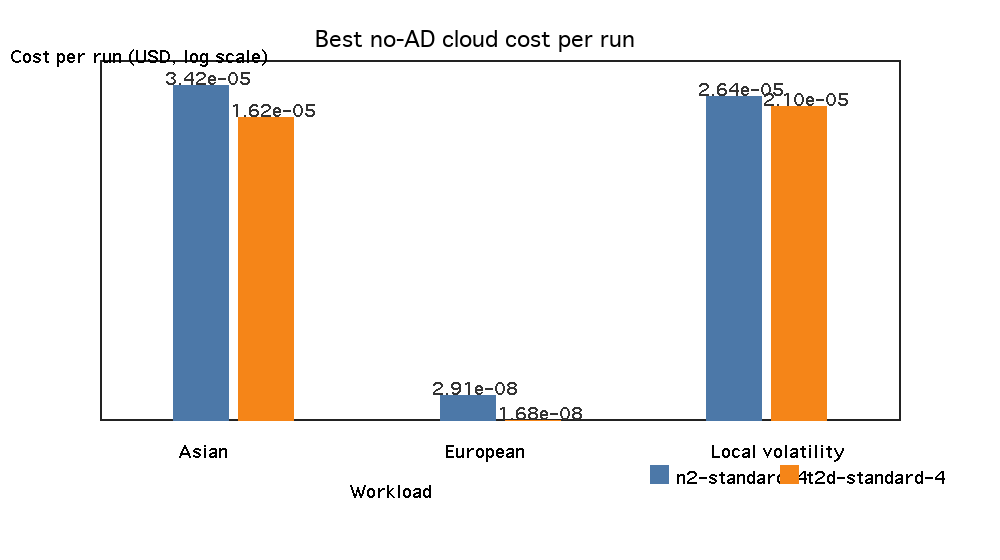
\includegraphics[width=\textwidth]{evaluation/figures/cloud_cost_performance_priced.png}
    \caption{Best no-AD cloud configurations at \(M=100{,}000\). The y-axis uses log-scale marginal compute cost per run; lower-left points indicate faster and cheaper measured configurations under the benchmark protocol.}
    \label{fig:cloud-cost-performance}
\end{figure}

\subsection{Pareto Frontier}
\label{subsec:cloud-pareto}

Figure~\ref{fig:pareto-runtime-cost} plots runtime against estimated cost for
the final \code{n2-standard-4} full-grid comparison. Because the plotted
configurations are on the same instance type, runtime and cost are closely
linked. The value of the Pareto analysis is therefore not that it reveals a
complex two-dimensional trade-off on one machine, but that it gives a precise
target for profiler recovery: a profiler should retain the configurations that
the full grid identifies as non-dominated under the measured metrics.

\begin{figure}[htbp]
    \centering
    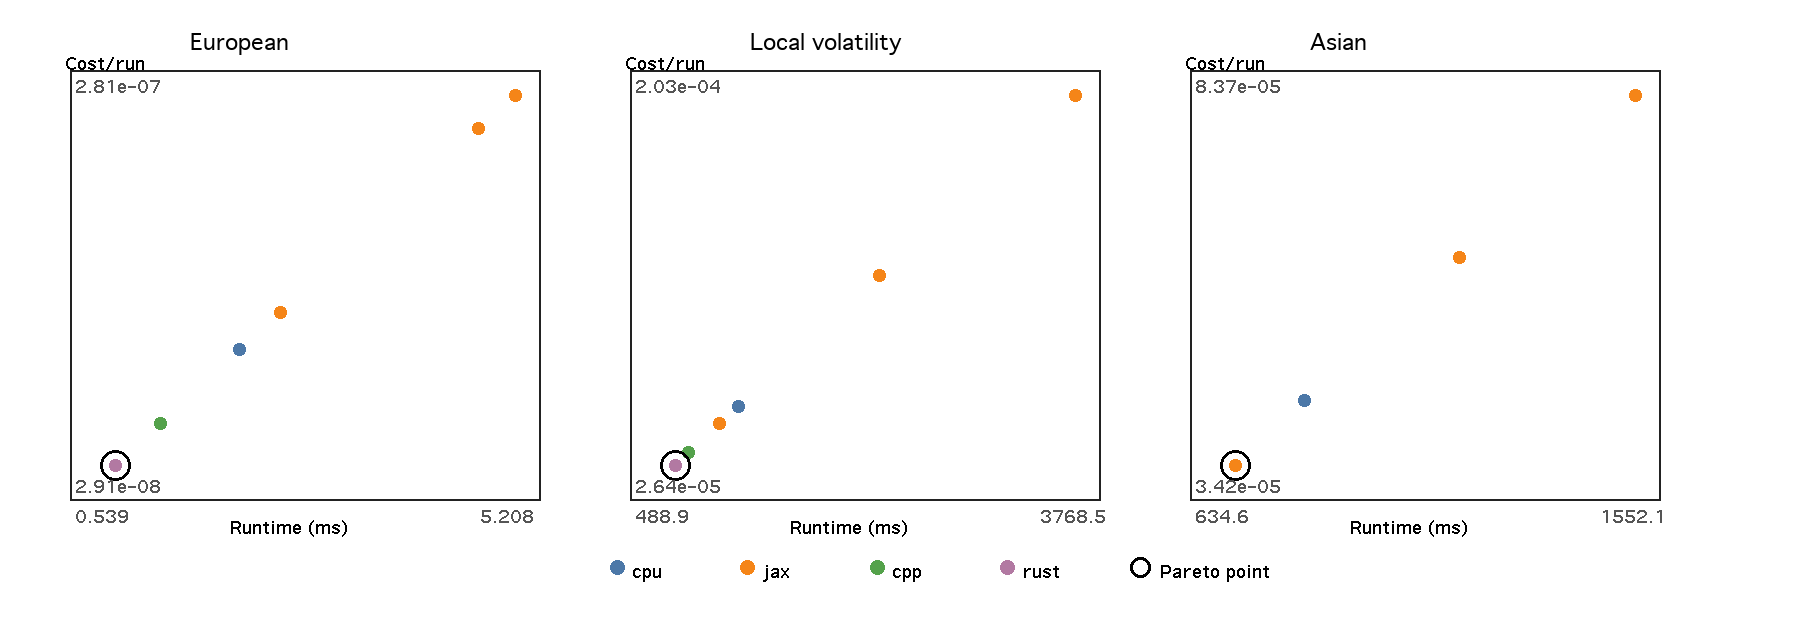
\includegraphics[width=\textwidth]{evaluation/figures/pareto_runtime_cost_n2.png}
    \caption{Runtime versus estimated cost for the final \code{n2-standard-4} grid. Pareto-optimal points are highlighted.}
    \label{fig:pareto-runtime-cost}
\end{figure}

\subsection{Old Profiler versus SHA}
\label{subsec:cloud-profiler-comparison}

Table~\ref{tab:profiler-comparison} is the main final cloud result. The full
grid contains 48 full benchmark runs. The old profiler selects 30 runs, saving
37.5\%. SHA selects 24 runs, saving 50.0\%. Both profilers recover 100.0\% of
the full-grid Pareto frontier and incur 0.0\% runtime and cost regret relative
to the full-grid best. SHA also achieves a stored final probe-to-full Spearman
rank correlation of 1.000, compared with 0.935 for the old profiler evidence.

\begin{table}[htbp]
\centering
\footnotesize
\setlength{\tabcolsep}{4pt}
\renewcommand{\arraystretch}{1.08}
\caption{Full-grid, old-profiler and SHA comparison for the final \code{n2-standard-4} cloud experiment. SHA preserves the full-grid decision on this slice while reducing full-scale runs.}
\label{tab:profiler-comparison}
\begin{tabularx}{\textwidth}{Yrrr}
\toprule
\textbf{Metric} & \textbf{Full grid} & \textbf{Old profiler} & \textbf{SHA} \\
\midrule
Candidate configurations & 16 & 16 & 16 \\
Full benchmark runs & 48 & 30 & 24 \\
Full runs saved & 0 & 18 & 24 \\
Percentage saved & 0.0\% & 37.5\% & 50.0\% \\
Pareto recovery & baseline & 100.0\% & 100.0\% \\
Runtime regret & baseline & +0.0\% & +0.0\% \\
Cost regret & baseline & +0.0\% & +0.0\% \\
Spearman $\rho$ probe--full & -- & 0.935 & 1.000 \\
Probe path-budget saving & -- & -- & 95.5\% \\
Mean scaling-law error & -- & -- & 9.7\% \\
\bottomrule
\end{tabularx}
\end{table}


This result is promising for the \code{n2-standard-4} slice, but it should not
be read as proof that SHA is generally reliable across workloads, instance
families, pricing snapshots, or noisy probe rankings. In the measured headline
grid, SHA halves the number of full-scale cloud benchmark cells while
preserving the full-grid decision quality on the reported metrics. The
practical significance is that the expensive part of the experiment is not
merely shifted elsewhere: the SHA probe path budget is 95.5\% lower than
evaluating the grid at full scale, and the mean scaling-law extrapolation
error is 9.7\%.

\subsection{Guarded SHA Local-Volatility Profiler}
\label{subsec:guarded-sha-localvol}

The robustness issue above motivated a guarded SHA experiment focused on the
local-volatility deployment problem. The candidate space is split into fair
task pools: an all-implemented-backends price-only pool, a validated-backend
price-only pool that excludes Rust because of the local-volatility price
discrepancy discussed in Section~\ref{subsec:limitations-localvol-correctness}, and an
AD-required pool comparing only configurations that produce Greeks. The run
evaluates five four-vCPU Google Cloud instance types
(\code{e2}, \code{n2}, \code{n2d}, \code{c2d}, and \code{t2d}) with \(M=1k\),
\(5k\), and \(25k\) probes and a \(100k\)-path full-grid oracle. The clean
combined artefact contains 120 observations.

\begin{table}[htbp]
\centering
\scriptsize
\caption{Guarded SHA local-volatility recommendations and pure runtime/cost baselines.}
\label{tab:guarded-sha-localvol}
\begin{tabularx}{\textwidth}{l l l l l r}
\toprule
\textbf{Pool/task} & \textbf{Objective} & \textbf{Weighted rec.} & \textbf{Fastest} & \textbf{Cheapest} & \textbf{Regret} \\
\midrule
All price-only & Speed & \code{rust/none/t2d} & \code{rust/none/c2d} & \code{rust/none/t2d} & 0.0\% \\
All price-only & Balanced & \code{rust/none/t2d} & \code{rust/none/c2d} & \code{rust/none/t2d} & 0.0\% \\
All price-only & Cost & \code{rust/none/t2d} & \code{rust/none/c2d} & \code{rust/none/t2d} & 0.0\% \\
Validated price-only & Speed & \code{cpp/none/t2d} & \code{cpp/none/t2d} & \code{cpp/none/t2d} & 0.0\% \\
Validated price-only & Balanced & \code{cpp/none/t2d} & \code{cpp/none/t2d} & \code{cpp/none/t2d} & 0.0\% \\
Validated price-only & Cost & \code{cpp/none/t2d} & \code{cpp/none/t2d} & \code{cpp/none/t2d} & 0.0\% \\
AD-required & Speed & \code{jax/reverse/t2d} & \code{jax/reverse/c2d} & \code{jax/reverse/t2d} & 0.0\% \\
AD-required & Balanced & \code{jax/reverse/t2d} & \code{jax/reverse/c2d} & \code{jax/reverse/t2d} & 0.0\% \\
AD-required & Cost & \code{jax/reverse/t2d} & \code{jax/reverse/c2d} & \code{jax/reverse/t2d} & 0.0\% \\
\bottomrule
\end{tabularx}
\end{table}

\begin{table}[htbp]
\centering
\scriptsize
\caption{Same-grid profiler comparison for the balanced guarded-SHA objective.}
\label{tab:guarded-sha-method-comparison}
\begin{tabularx}{\textwidth}{l r r l r r r l}
\toprule
\textbf{Method} & \textbf{Used} & \textbf{Saved} & \textbf{Selected config.} & \textbf{Obj.} & \textbf{Run} & \textbf{Cost} & \textbf{Validity status} \\
\midrule
Full-grid oracle & 30 & 0 & Price: \code{rust} perf./\code{cpp} valid; AD: \code{jax} & 0.0\% & 0.0\% & 0.0\% & Reference grid \\
Plain SHA & 7 & 23 & Price: \code{rust} perf./\code{cpp} valid; AD: \code{jax} & 0.0\% & 0.0\% & 0.0\% & Less guarded \\
Guarded SHA & 17 & 13 & Price: \code{rust} perf./\code{cpp} valid; AD: \code{jax} & 0.0\% & 0.0\% & 0.0\% & Preferred policy \\
\bottomrule
\end{tabularx}
\end{table}


Table~\ref{tab:guarded-sha-localvol} shows a stronger and more defensible
profiler story than the unguarded SHA audit. The repeated \code{t2d} selection
is not a transcription error: the objective is a weighted runtime--cost score,
not pure elapsed time. \code{c2d} is the fastest pure runtime choice, but
\code{t2d} is only 6.0\% slower and 24.3\% cheaper for price-only, and 4.9\%
slower and 25.5\% cheaper for AD-required. This is enough for \code{t2d} to win
even the speed-sensitive 0.8/0.2 objective.

The all-backend price-only pool selects \code{rust/none/t2d}, but this is a
performance recommendation only. Because Rust local-volatility pricing has not
passed the same cross-engine consistency check as NumPy, C++ and JAX, the
validated price-only deployment recommendation is instead
\code{cpp/none/t2d}. The AD-required recommendation is
\code{jax/reverse/t2d}; these local-volatility sensitivities are internally
consistent JAX AD outputs rather than closed-form-validated Greeks.

The 0.0\% regret values are measured against the observed full-grid oracle for
this tested local-volatility configuration, candidate engines, AD modes,
instance types and \(100k\)-path target budget. They do not imply the true
global optimum over all cloud instances, thread counts, workloads or larger path
budgets. Table~\ref{tab:guarded-sha-method-comparison} shows that plain SHA
also recovers the observed oracle on this grid while selecting fewer full runs;
guarded SHA is reported as the safer policy because it trades some of that
saving for explicit near-tie, engine-diversity, instance-family and
scaling-improvement safeguards. Cloud timing variation means the small
\code{c2d}/\code{t2d} gaps should be interpreted as near-tie deployment
evidence rather than permanent hardware rankings.

\subsection{SHA Progression in the Earlier Multi-Workload Grid}
\label{subsec:sha-progression}

This subsection returns to the earlier multi-workload
\code{sha\_cloud\_profiler\_v4} experiment and visualises the promotion path on
the \code{n2-standard-4} grid. Figure~\ref{fig:sha-progression} shows that all
16 configurations are evaluated at the cheapest probe level, then the active
set is reduced as the path budget increases. The final selected set contains
the configurations promoted for full benchmarking after the profiler's
conservative safeguards are applied.

\begin{figure}[htbp]
    \centering
    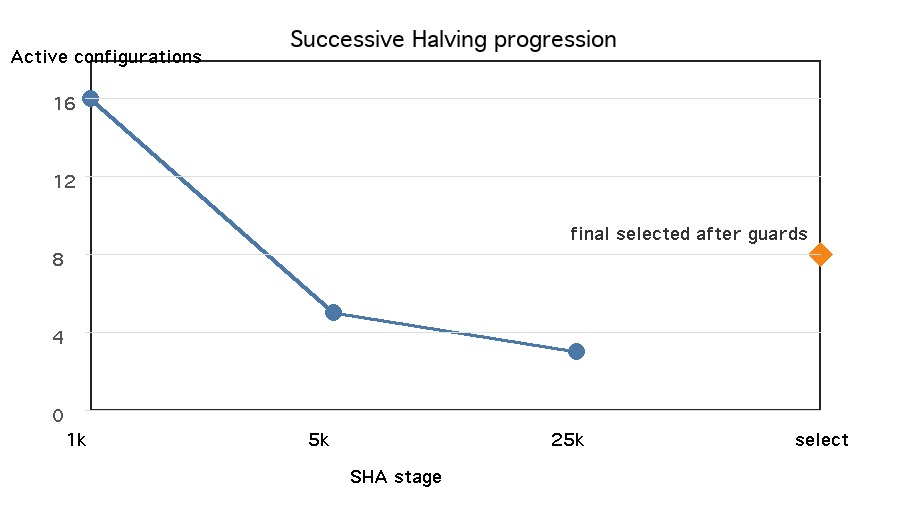
\includegraphics[width=0.95\textwidth]{evaluation/figures/sha_progression_n2.png}
    \caption{SHA promotion path on the earlier \code{n2-standard-4} multi-workload grid. Most configurations receive only cheap probes, while the active set shrinks as the path budget increases.}
    \label{fig:sha-progression}
\end{figure}

The progression illustrates why SHA is useful in this setting. Most
configurations receive only cheap measurements, while promising configurations
receive more budget. In the final experiment this is enough to identify the
same best runtime configuration as the full grid:
\code{rust/european/none} at \(M=100{,}000\), with runtime \(0.54\) ms.

\section{Cross-Question Discussion}
\label{sec:results-discussion}

\subsection{Software Stack and Engine Performance}
\label{subsec:discussion-software-stack}

The local-volatility results show that engine choice has a substantial effect
on throughput.  Rust/Rayon is the fastest no-AD engine by runtime across the main
\(M\)-sweep and the large stress test.  At \(M=500k\), \(N=252\), Rust is
about \(2.1\times\) faster than NumPy and about \(1.25\times\) faster than
JAX or C++.  JAX and C++ are very similar at larger local-volatility sizes,
while NumPy remains consistently slower.

The result also shows why the European GBM workload should not be treated as
the main benchmark.  On the small GBM baseline, C++ was clearly dominant.
On local volatility, Rust becomes fastest and JAX becomes competitive with
C++.  This demonstrates that engine rankings depend strongly on workload
structure.

The numerical interpretation is more cautious. The independent uncertainty
check indicates that NumPy, C++ and JAX agree within estimated Monte Carlo
error on the local-volatility price, while Rust does not. Thus Rust is best
interpreted here as evidence for the throughput available from a Rayon-based
native implementation, not as a fully validated local-volatility pricing
backend.

\subsection{Programming-Language, Runtime and AD-Support Trade-offs}
\label{subsec:discussion-language-ad}

The compiled CPU engines provide the strongest no-AD local-volatility
runtime performance.  Rust/Rayon performs best overall in the local-volatility
timing experiments, while C++/OpenMP remains competitive and scales well with
threads.  JAX/XLA is not the fastest no-AD engine, but it provides the main
AD capability and becomes close to C++ on larger multi-step workloads.

This should not be read as a broad benchmark of AD libraries across languages.
The completed implementation compares JAX forward- and reverse-mode AD against
native no-AD engines in NumPy, C++ and Rust. The C++ and Rust engines are
valuable systems baselines, but they do not evaluate C++ AD tools, Rust AD
libraries, Enzyme, or source-transformation AD in those languages.

The AD results show a clear trade-off.  Reverse-mode AD is consistently much
faster than forward-mode AD for the scalar-output local-volatility pricing
function, with reverse-mode overhead usually around \(2.1\)--\(2.6\times\)
and forward-mode overhead around \(4\)--\(7\times\).  However, reverse mode
also reaches memory limits at larger \(M,N\) combinations.  Therefore, the
best AD choice depends on whether the bottleneck is runtime or memory.

\subsection{Parallelism and Bottlenecks}
\label{subsec:discussion-parallelism}

The thread-scaling results show that C++ and Rust expose path-level
parallelism effectively to OpenMP and Rayon.  Rust achieves \(3.66\times\)
strong-scaling speedup at four requested threads and \(3.68\times\)
weak-scaling throughput speedup.  C++ also scales well, though less strongly,
with \(3.09\times\) strong-scaling speedup and \(3.11\times\) weak-scaling
throughput speedup.

JAX behaves differently.  It is competitive in absolute runtime for no-AD
local-volatility execution, but it does not respond to requested thread-count
changes.  This indicates that XLA's managed CPU runtime should be interpreted
separately from explicit OpenMP/Rayon thread scaling.  For this project, the
main bottlenecks are therefore different by engine: compiled engines are
limited by parallel efficiency and memory bandwidth at higher thread counts,
while JAX is limited by its managed execution model and, for reverse-mode AD,
by memory pressure.

\subsection{Compiler and AD Runtime Techniques}
\label{subsec:discussion-ai-techniques}

The JAX/XLA results provide evidence for the relevance of compiler and AD
runtime techniques to Monte Carlo simulation.  JAX is relatively weak on the
small European GBM baseline, but becomes competitive with C++ on the
multi-step local-volatility workload.  This suggests that XLA-style compiled
execution becomes more attractive when the workload has enough repeated
structure to amortise dispatch and compilation overheads. The conclusion is
therefore limited but useful: in this project, JAX/XLA is most valuable as an
AD-capable compiled backend rather than as a universally fastest no-AD engine.

\subsection{Integrated Scope of the Completed Evaluation}
\label{subsec:discussion-scope}

The completed experiments strongly address local MC+AD benchmarking,
programming-language comparison, AD overhead, memory/resource limits, thread
scalability, and a targeted form of cloud resource selection. The final
cloud-profiler study adds measured cost-performance, Pareto-frontier, and
profiler-selection evidence.

This scope is scientifically useful. The project demonstrates a reproducible
benchmarking framework that can run multiple engines under matched workload
definitions, capture repeated measurements, evaluate AD overheads, reveal
practical resource limits, and attach cloud cost metadata to final selection
decisions. The local-volatility suite also shows that more realistic MC+AD
workloads can change the conclusions drawn from simple one-step baselines.

\section{Limitations and Threats to Validity}
\label{sec:results-limitations}

\subsection{Hardware and Cloud Scope}
\label{subsec:limitations-single-machine}

The detailed scaling and memory experiments were collected on a single
Codespace environment. This makes the comparisons controlled and reproducible
under the recorded conditions, but it prevents broad claims about AMD versus
Intel, workstation versus cloud, or CPU versus GPU performance. The final cloud
experiments add targeted Google Cloud evidence, but those results are still
tied to specific instance types, regions, prices, software versions, and run
dates. They should therefore be interpreted as measured cost-performance
evidence for the reported configurations, not as universal cloud hardware
rankings.

\subsection{Local-Volatility Correctness}
\label{subsec:limitations-localvol-correctness}

The European GBM workload has a closed-form Black--Scholes reference, but
the chosen parametric local-volatility workload does not.  Local-volatility
correctness is therefore assessed through cross-engine consistency and
convergence with larger \(M\), rather than by exact analytical error.  The
additional high-\(M\) uncertainty check quantifies this limitation: NumPy, C++
and JAX agree within estimated Monte Carlo error, while Rust does not. For that
reason, Rust local-volatility results are retained as throughput and scaling
evidence, but Rust is not treated as a correctness-certified local-volatility
pricing backend in the guarded-profiler deployment recommendation. Price
differences between engines may reflect different random-number generators,
path-generation implementations, or, in the Rust case, a backend-specific
issue that requires further investigation. Likely causes include RNG stream
partitioning, per-thread path assignment, discretisation mismatch, or a
payoff/discounting implementation difference. A future validation step should
use deterministic per-path random streams shared across engines and compare
pathwise terminal values before comparing aggregate prices.

The AD correctness story is similarly scoped. European GBM prices and Greeks
are analytically validated against Black--Scholes. Local-volatility prices are
validated by cross-engine agreement and convergence where possible, but
local-volatility Greeks have no closed-form reference in this report. The
reported local-volatility sensitivities are therefore checked as internally
consistent JAX AD outputs, not as analytically validated Greeks. A finite-difference check using common random numbers would be the most useful
next validation step for the reported JAX local-volatility Greeks.

\subsection{Random Number Generation as a Confounder}
\label{subsec:limitations-rng}

The engine comparisons measure complete backend implementations rather than
isolated path-evolution kernels. This is useful for deployment because random
number generation is part of real Monte Carlo runtime, but it also means the
measured differences between NumPy, JAX, C++ and Rust combine simulation-kernel
cost, RNG cost, memory layout, and reduction behaviour. The current results do
not separate these effects. A stronger microbenchmark would run a
pre-generated-normal experiment in which all engines consume the same normal
variates, allowing RNG generation to be separated from path evolution and
payoff reduction.

\subsection{Warm versus Cold JAX Execution}
\label{subsec:limitations-cold-warm}

The main timing tables report warm steady-state runtimes after configured
warmup repetitions. This is appropriate for repeated production-style
simulation and for comparing amortised kernel execution, but it is optimistic
for short-lived cloud jobs where JAX/XLA compilation may be paid on the
critical path. The implementation records and discusses compilation effects,
but the final cloud cost-performance tables do not include a full cold-start
versus warm-start comparison. Therefore, cloud cost claims should be read as
steady-state cost-performance rather than one-off job latency.

\subsection{Cloud Cost Scope}
\label{subsec:limitations-cloud-cost}

The cloud-cost estimates use marginal compute cost only. They intentionally
exclude startup and shutdown time, idle time, persistent storage, orchestration
overhead, retries, network transfer and billing granularity. This is defensible
for comparing measured configurations under the same benchmark protocol, but it
should not be interpreted as an exact Google Cloud invoice or as a complete
end-to-end deployment-cost model.

\subsection{Memory Measurement}
\label{subsec:limitations-memory-measurement}

Process-level memory measurements are coarse, especially for JAX/XLA, which
may cache allocations or materialise intermediates inside compiled execution.
For this reason, small RSS deltas are not over-interpreted.  The OOM events
are treated as stronger evidence than individual low memory-delta readings.

\subsection{Thread Control}
\label{subsec:limitations-thread-control}

Thread-count control is more direct for C++/OpenMP and Rust/Rayon than for
JAX/XLA.  JAX uses its own CPU execution runtime, so requested OpenMP-style
thread counts do not translate into clean JAX scaling experiments.  This is
why JAX thread results are interpreted as runtime behaviour rather than as a
controlled thread-count benchmark.

\section{Summary}
\label{sec:results-summary}

Overall, the results show that MC+AD performance depends on workload structure,
runtime system, differentiation mode, parallel execution model and cloud cost
assumptions. European GBM validates prices and JAX Greeks against
Black--Scholes, while the local-volatility suite exposes the main runtime, AD,
memory and scaling trade-offs. Rust/Rayon gives the fastest measured no-AD
local-volatility timings, but its local-volatility price discrepancy means those
rows are performance evidence rather than correctness evidence. JAX provides the
main AD evidence: reverse mode is faster than forward mode for moderate
scalar-output local-volatility workloads, but reaches memory limits at larger
\(M,N\) combinations.

The cloud results show that marginal cost-performance can differ from raw
runtime ranking. Plain SHA halves full-grid work on the favourable
\code{n2-standard-4} slice, while the guarded local-volatility profiler matches
the observed oracle across the five-instance grid and avoids 13 of 30
full-scale task-level runs. These profiler results are promising, but scoped to
the measured grids and should be read together with the limitations above.


%% =========================
%% CHAPTER 7: CONCLUSION
%% =========================
\chapter{Conclusion}
\label{chap:conclusion}

\section{Summary of Work}

This project designed, implemented, and evaluated a reproducible benchmarking
framework for Monte Carlo option-pricing engines with automatic
differentiation. The framework supports explicit workload configurations,
engine abstraction, deterministic seeding, warm-up and repeated timing,
analytical validation where available, SQLite result storage, environment
metadata capture, cloud cost metadata, and generated report artefacts.

The completed implementation compares NumPy, JAX/XLA, C++/OpenMP, and
Rust/Rayon engines across European GBM, parametric local-volatility, and Asian
option workloads where supported. The local experimental campaign provides
detailed evidence on validation, runtime, throughput, AD overhead,
path-count scaling, time-step scaling, thread scaling, memory pressure,
surface-shape sensitivity, and timing stability. The final cloud experiment
extends this with cost-performance analysis, Pareto-frontier analysis, and
profiler-versus-grid evaluation.

\section{Key Findings}

The results show that MC+AD performance cannot be reduced to a single backend
ranking. The simple European GBM workload is useful for correctness checks, but
the more demanding local-volatility and Asian workloads change the observed
trade-offs. Rust/Rayon is the strongest no-AD engine in the main
local-volatility results and in the highlighted European/local-volatility cloud
rows, while JAX/XLA remains essential for AD and is competitive for some
path-dependent configurations.

The AD results show a clear runtime-memory trade-off. Reverse-mode AD is
substantially cheaper than forward mode for the scalar-output
local-volatility workload at moderate sizes, but it reaches practical memory
limits at larger \(M,N\) combinations. In the final cloud comparison at
\(M=100{,}000\), JAX AD overhead ranges from \(1.81\times\) for Asian reverse
mode to \(4.42\times\) for local-volatility forward mode.

The cloud-profiler result is the strongest final systems contribution. In the
\code{sha\_cloud\_profiler\_v4} experiment on \code{n2-standard-4}, the full
grid requires 48 full benchmark cells. SHA selects 24, saving 50.0\% of full
runs while preserving 100.0\% Pareto recovery and 0.0\% runtime and cost regret
relative to the full grid. The old profiler also preserves the best decisions,
but selects 30 full runs, so SHA achieves the same measured decision quality
with fewer full-scale evaluations.

\section{Answering Research Questions}

\paragraph{Hardware and software stacks.}
The local and cloud results show that runtime depends strongly on workload
structure, engine implementation, and runtime system. Compiled CPU engines are
very strong for no-AD workloads, while JAX/XLA is necessary for the reported AD
measurements and can be competitive when the workload has enough structure to
benefit from compilation.

\paragraph{Programming languages and AD libraries.}
C++/OpenMP and Rust/Rayon provide high no-AD throughput and explicit CPU
parallelism. JAX provides the main AD capability and exposes the practical
difference between forward and reverse mode. The trade-off is therefore not
only language performance, but also derivative support, memory behaviour, and
ease of integration into a reproducible benchmark runner.

\paragraph{Cloud cost-performance.}
The final priced comparison shows that runtime and cost should be considered
together. For the measured no-AD rows at \(M=100{,}000\),
\code{t2d-standard-4} is faster and lower cost per run than
\code{n2-standard-4}. This is a measured result under the stored pricing and
environment assumptions, not a universal claim about all cloud hardware.

\paragraph{AI/ML techniques.}
JAX/XLA demonstrates that compiler and AD techniques from the AI/ML ecosystem
are relevant to MC workloads, especially when the computation is expressed in a
form such as \code{jax.lax.scan} that the compiler can optimise. The project
does not complete mixed precision, GPU auto-tuning, or broader hardware-aware
scheduling experiments, so the conclusion is deliberately limited to the
measured XLA and AD evidence.

\paragraph{Parallelism and bottlenecks.}
The thread-scaling experiments show effective scaling for C++ and Rust under
OpenMP/Rayon-style parallelism, while JAX's CPU runtime is less directly
controlled by requested thread counts. The stress tests show that memory, not
only arithmetic throughput, becomes a limiting factor for reverse-mode AD on
large local-volatility workloads.

\section{Future Work}

The most direct next step is to broaden the cloud study. More instance types,
regions, repeated cloud runs, and up-to-date pricing snapshots would test
whether the SHA profiler remains reliable on larger and noisier grids. The
profiler could also incorporate uncertainty estimates so that promotion
decisions account explicitly for timing variance and Monte Carlo noise.

GPU execution, distributed execution, mixed precision, and hardware counters
remain important extensions. The framework already has a CUDA scaffold and
metadata structure, but the final evaluation does not claim GPU results.
Extending the benchmark suite to GPUs and distributed workers would make the
hardware-comparison part of the original proposal much stronger.

Further AD systems and languages would also be valuable. The project evaluates
JAX AD, but future work could compare Enzyme, C++ AD tools, Rust AD libraries,
Mojo, or domain-specific quant libraries. Finally, the frontend and API could
be developed into a more complete dashboard for interactive profiler
configuration and report artefact generation.

\section{Final Remarks}

Overall, the project contributes both a working engineering artefact and an
empirical methodology. The artefact makes MC+AD experiments reproducible,
queryable, and extensible across engines. The methodology shows how detailed
local benchmarking can be combined with cloud cost metadata and successive
halving to reduce expensive full-grid benchmarking while preserving measured
selection quality. The final report therefore represents an expanded and
completed version of the original framework work: it retains the detailed
technical and experimental narrative, while adding the final cloud,
cost-performance, Pareto-frontier, AD-overhead, and SHA-profiler results.


%% =========================
%% DECLARATIONS
%% =========================
\chapter*{Declarations}
\addcontentsline{toc}{chapter}{Declarations}

\section*{Academic Integrity}

This report is submitted as my own work. External sources, software libraries,
and project guidance have been acknowledged where used. The implementation,
experimental design, analysis, and final interpretation were reviewed and
assembled by the author.

\section*{Generative AI Assistance}

Generative AI tools were used as writing and coding assistants during parts of
the project, including for drafting support, proofreading, code explanation,
and editing suggestions. All AI-assisted material was critically reviewed,
checked against the project repository, benchmark artefacts, and generated
tables or figures, and edited by the author before inclusion. Numerical claims
in the report are based on stored benchmark results and generated report
artefacts rather than unsupported model output. The final interpretation,
selection of evidence, and responsibility for the submitted work remain mine.


%% Appendix material is submitted as supporting artefacts in the repository;
%% it is omitted from the main PDF to stay within the page limit.

\bibliographystyle{unsrt}
\bibliography{bibs/sample}

\end{document}
